\documentclass[]{final_report}
\usepackage{graphicx}
\usepackage{hyperref}
\usepackage[final]{pdfpages}
\usepackage{booktabs}
\usepackage{multirow}
\usepackage{framed}
\usepackage{caption}
\usepackage{subcaption}
\usepackage{tikz}
\usepackage{xcolor}
\usetikzlibrary{timeline}
\usepackage{dirtree}
\setlength\parindent{24pt}
\usepackage[newfloat]{minted}
\usepackage{wrapfig}

\newenvironment{mycode}{\captionsetup{type=listing}}{}
\SetupFloatingEnvironment{listing}{name=Source Code}

%%%%%%%%%%%%%%%%%%%%%%
%%% Input project details
\def\studentname{James King}
\def\reportyear{2018}
\def\projecttitle{Cooperative Strategies in Multi-Agent Systems}
\def\supervisorname{Kostas Stathis}
\def\degree{BSc (Hons) in Computer Science}
\def\fullOrHalfUnit{Full Unit} % indicate if you are doing the project as a Full Unit or Half Unit
\def\finalOrInterim{Final Report} % indicate if this document is your Final Report or Interim Report

\begin{document}

\maketitle

\chapter*{Declaration}

This report has been prepared on the basis of my own work. Where other published and unpublished source materials have been used, these have been acknowledged.

\vskip3em

Word Count: 1,587 \textit{2,000} intro + n \textit{3,000} lit review + n \textit{4,000} framework + n \textit{4,000} experiment evaluation + n \textit{1,000} conclusions + n \textit{1,000} professional issues

\vskip3em

Student Name: \studentname

\vskip3em

Date of Submission: \today

\vskip3em

Signature: 
\includegraphics[scale=0.05]{Signature.png}

\newpage

%%%%%%%%%%%%%%%%%%%%%%
%%% Table of Contents
\tableofcontents\pdfbookmark[0]{Table of Contents}{toc}\newpage

%%%%%%%%%%%%%%%%%%%%%%
%%% Your Abstract here

\begin{abstract}
\end{abstract}
\newpage

\chapter{Introduction}
Artificial intelligence (AI) has been an idea present in the consciousness of humanity for millennia. From Hephaestus' mighty Talos to Edgar Allan Poe's commentary on `Maelzel's Chess-Player' the idea has inspired both awe and confusion. As we move away from the mythical and the false, AI embeds itself deeper into our lives and societies. AI techniques are being used for many novel applications in areas such as medicine~\cite{glaucoma} and game playing~\cite{alphago}.\par
Many of these applications are specifically using agent techniques~\cite{silverman2015systems, mvfcec, brockman2016openai}. Intelligent agents (IAs) have many definitions but one popular definition is that agents are anything that perceives and acts upon its environment~\cite{russell2016artificial}. Agents are situated in an environment and many of these agents can be combined in one environment to form a multi-agent system (MAS).

\section{Motivation}
Within MASs it is generally possible for the agents to interact and/or to communicate with each other. Communication generally occurs through agent communication languages (ACLs). The interactions that occur between agents are actions by one or all of the agents in the interaction. There is a possibility that agents can act out of pure altruism and always cooperate with other agents. However, often agents will work to protect their interests i.e. they are selfish.\par
It is desirable for agents in a MAS to work together to complete tasks and fulfil goals. Therefore, we want to facilitate cooperation between agents which may be selfish. There are analytical tools that we can use in game theory to understand what happens when decision-making individuals interact~\cite{myerson2013game}. Some of these tools are used to explain how cooperation occurs between selfish individuals.\par
Many of these tools rely on the idea of reciprocal altruism~\cite{trivers1971evolution}, which stipulates that cooperation can occur between selfish individuals if they expect cooperation to be reciprocated. Two such mechanisms are direct and indirect reciprocity. Indirect reciprocity refers to when an agent cooperates with another agent with the expectation that this cooperation will increase the chance of receiving cooperation from others later. Direct reciprocity on the other hand, refers to the expectation of reciprocating cooperation from the agent who initially received the cooperation.\par
There are many factors to consider surrounding the mechanism. One key factor is the level of visibility of the interactions within the MAS. Nowak and Sigmund~\cite{evol_indirect_image} limit this visibility to a randomly selected group of individuals in the population (onlookers). Another factor to consider is how information about the interactions can be conveyed. Sommerfeld \textit{et al.} suggested the use of gossip~\cite{gossip_alt}.\par 
So how can we use these mechanisms to facilitate cooperation between IAs? What options can we use and how can we make use of them to encourage cooperation between these agents?

\section{Aims and Objectives}
\label{sec:aao}
The high level aim of this project is to study how game-theoretic techniques can be leveraged in MASs to create cooperative societies of agents. Derived from this high level aim the objectives of this work are to develop a theoretical framework/model using game-theoretic and MAS techniques inspired by past work in both fields. The next is to implement this framework in a MAS that allows transparent decision making by agents; by which I mean that agents are able to give reasons for their decisions. Another objective is to build this implementation on a distributable platform that allows users to set up games of the model, specify certain variables and view an analysis of the game in order to study how the mechanism and variables affect cooperation in the system.\par
A feature of the system will be that users are able to create an account and refer back to games they have previously run. I will be using the system and specifically this feature to run my own experiments in order to study the effectiveness of the techniques I have employed and to discover how the system needs to be set up in terms of the variables present. I will then present these experiments and discuss the results with a conclusion on my findings and suggestions of future work as a result of these findings.\par
Objectives:
\begin{enumerate}
	\item Develop a theoretical framework
	\item Implement this framework
	\item Run experiments using the implementation
	\item Analyse the experiments and evaluate the results
\end{enumerate}

\section{Contribution}
Much of the work I have reviewed in relation to game-theoretic mechanisms has come from the field of game theory. Because the studies have come from game theorists the implementation of the models devised by the authors have not generally used MAS techniques. My implementation is not only a MAS using a game-theoretic model, but it supports transparent agent decisions due to the use of the logic programming language Prolog for the implementation of agents' decision making components. This implementation is also a web based system, allowing users across the world to experiment with the model I have devised.\par
Furthermore, the theoretical framework I have designed is inspired by past work on game-theoretic mechanisms, but also builds upon these approaches. One way in which I build upon these is by combining the many aspects of the past approaches such as using MAS techniques to create a game-theoretic model (combining direct and indirect reciprocity) and using gossip as an action to convey reputation information in a mixed reciprocity model.\par
Lastly, in my system, users associate agents with specific strategies which I have included in the system. These strategies come from past work in the topic of game theory, but are implemented using an agent architecture which I have purpose-designed for my theoretical framework. This arhcitecture included augmenting the original strategies with strategy components for whatever roles agents may have at a particular time-point in a society (such as when an agent is not in an interaction). Another development is the trust models which I have created for the original strategies for interpreting the events in the environment.

\section{Structure}
In the next chapter of this report I have explored and described the past work that has been a central inspiration to the theoretical framework I have devised. I have included other interesting information and possible mechanisms from past work that could be used to encourage cooperation in MASs in the appendix. This background reading then leads into the next chapter in which I have defined the theoretical framework for my system.\par
Following on from the theoretical framework in the same chapter, I have described the implementation of this theoretical framework in a web application. This application is available for users across the internet to set up games and view the events and analysis of their games. In the next chapter, I use this platform to experiment in order to review the effectiveness of the mechanism, strategies and variables in the game in encouraging cooperation between selfish agents.\par
The final two main chapters of this report discuss my findings from the experiments and rest of the project. I then conclude and evaluate the project. The appendix is at the end and contains further information referenced in the report but which is not necessarily central to the project.

\chapter{Background}

\section{Introduction}
In the following sections of this chapter I will be exploring and describing past work relevant to this project including MAS techniques and related studies in game theory. First I will describe MAS techniques and concepts that are important to this project including subsections on agents, an agents environment and agent communication. Secondly I will discuss game-theoretical approaches to modelling and studying multi-agent interactions in regards to the evolution of cooperation in MASs.

\section{Multi-Agent Systems and Intelligent Agents}
\label{sec:backgroundmas}
MASs are a field in computer science concerning the development of societies of agents in which agents are computer systems are computer systems that are capable of deciding on what actions to take in order to reach a delegated goal or the agent's design objectives~\cite{wooldridge2009introduction}. These agents typically interact using agent communication languages (ACLs).\par 

\subsection{Environments}
Russell and Norvig~\cite{russell2016artificial} state that an agent is designed to work in an environment class or a set of environments. According to Wooldridge~\cite{wooldridge_jennings_1995} an agent is built to fulfil design objectives. These design objectives work within the restriction of the agents environment. Following from this Russell and Norvig~\cite{russell2016artificial} define an agent in terms of it's environment, stating that an agent is any system that uses sensors to perceive it's environment and effectors to act upon it's environment.\par
\begin{wrapfigure}{l}{0.5\textwidth}
\vspace{-20pt}
\begin{framed}
	\center
	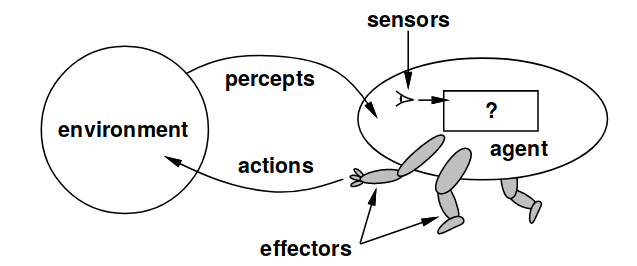
\includegraphics[width=\textwidth]{russellnorvigagent.png}
	\caption{Russell and and Norvig's~\cite{russell2016artificial} agent}
	\label{fig:rnagent}
\end{framed}
\vspace{-20pt}
\end{wrapfigure}
A generic program was designed by Russell and Norvig~\cite{russell2016artificial} for how an environment program should run in which there are steps that run in a cycle. In the first step, perception of the environment occurs for each agent in which the agent can use it sensors to receive percepts from the environment. In the next step agents all decide on an action. After all have decided the state of the system is then changed based on the actions that the agents have decided on. A fourth step was added to update the performance scores of each agent.\par 
The effect of these cycle steps is to keep agents synchronised preventing agent actions from changing the state of the environment while other agents are deliberating. A static environment is one that does not change whilst an agent is deliberating. Dynamicity is one of Russell and Norvig's~\cite{russell2016artificial} five properties of an environment. The synchronicity of this generic environment program helps keep the environment static, unless other forces (not agent actions) have an effect on the environment's state.\par 
The opposite to a static environment is a dynamic one, in which the environment can change during decision making. Another environment property is accessibility. An accessible environment is one that gives an agent full access to the state of that environment. In an accessible environment there is no need for an agent to keep any internal state about the environment. Unlike in inaccessible environments, in which an agent cannot simply sense all aspects of that environment that are relevant for decision making.\par 
A third property from Russell and Norvig~\cite{russell2016artificial} is whether the environment is episodic or not. An episodic environment is split into episodes where the quality of actions in each episode do not depend on previous episodes.\par 
These properties determine how complex an environment is. The final two are whether the environment is deterministic or not and whether the environment is continuous or discrete. If an environment is deterministic it means the effects of an action given some conditions is guaranteed. If an agent can access the whole state of the environment (accessibility) and the environment is deterministic the agent can guarantee the outcome of their action.\par 
An environment is considered discrete actions and percepts are clearly defined and there are a limited number of them. The more properties of an environment that match the following properties, the more complex the environment: continuous, non-deterministic, inaccessible, dynamic, non-episodic.\par 

\subsection{The Agent Model}
Yoav Shoham introduced the agent-oriented programming (AOP) paradigm~\cite{shoham1993agent}. This paradigm is similar to object-oriented programming (OOP). In Shoham's formulation of AOP~\cite{shoham1991agent0} object units are replaced agents, the internal state of a unit is constrained to beliefs, commitments and capabilites, message passing is constrained to using speech act theory to communicate and constraints are placed on methods.
\subsubsection{What is an agent?}
Since Shoham's formulation there has been much debate as to whether systems are agent systems or simply programs~\cite{franklin1996agent}. The exact definition of agency varies depending upon which source is consulted and the application of the concept.\par 
Wooldridge and Jennings~\cite{wooldridge_jennings_1995} gave one of the most influential and powerful descriptions. They put forward a weak notion of agency by laying out four main properties: autonomy, social ability, reactivity and pro-activeness.\par 
Autonomy refers to agents having control over their actions and internal state, and operating without outside intervention. Social ability is the use of an ACL to interact with other entities such as humans and other agents. Responding to environment changes in a timely fashion is what the property of reactivity refers to. Finally pro-activeness is the display of taking initiative to work towards a goal, not simply in reaction to environmental state changes.\par 
Wooldridge and Jennings go on to note that stronger notions of agency endow agents with human-like mental notions. These mental notions represent information in a symbolic model, and make decisions by reasoning with this symbolic model in a symbolic way. This representation and reasoning is no easy feat - known as the representation/reasoning problem~\cite{wooldridge2009introduction} - but it does allow agents to make explainable and transparent decisions.\par 
A more up to date and stronger notion of agency may include the use of new developments such as computer vision, natural language processing and deep reinforcement learning concepts. Stronger notions of agency show a tendency towards more humanlike characteristics and AI concepts, drawing clear comparison with a long term goal of AI: to produce systems capable of beating The Imitation Game~\cite{machinery1950computing}.
\subsubsection{Russell and Norvig's Agent Program Components}
Russell and Norvig~\cite{russell2016artificial} formulated a number of agent program models to describe the internal make up of agents that allow an agent to act in and understand their environment.\par
The first model is simple reflex agents which keep no internal state, they simply use their percepts from the environment and condition-action rules to decide on actions. These are comparable to reactive agent architectures. Model-based reflex agents use percepts from their environment to form a state which to use alongside condition-action rules and a model of how the state of their world evolved to make decisions.\par 
Goal and utility-based focus on the drives of an agent. The goal based architecture keeps an internal state, and combines this with search and planning decision making components to reach specified goals. States in which an agent is more successful can be formulated in terms of having a higher utility. Utility based agents work to maximise that utility, even in situations when an agent has conflicting goals in which the utility is formed by creating a tradeoff between the conflicting goals.
\subsubsection{Learning Agents}
Learning agents is the final agent model described by Russell and Norvig. Programs created using this model are not formed by a programmer specifying how to act. Instead these agents use a number of components to feed into a decision making system (performance element). Feedback is provided by the critic component to the learning element which makes changes to the performance element. The problem generator is another component that suggests actions that will hopefully lead to new knowledge.\par 
Machine learning is exploding with new concepts and developments, most notably from the agents systems persepctive deep reinforcement learning. Agents using machine learning techniques often appear to satisfy stronger notions of agency. However, these techniques do not come from a symbolic AI background, and lead to a lack of explainability.\par 
Unifying these techniques with symbolic AI approaches to produce agents which can explain their decisions in order to produce verifiable systems is a keenly researched topic~\cite{darpaxai, garnelo2016towards}. However, this is an even tougher version of the representation/reasoning problem as we are not only trying to reason with symbolic data, but reason in a complex manner with deeply mathematical techniques.
\subsubsection{Deductive Reasoning Agents}
Deductive reasoning agents use a form of symbolic AI. The symbolic representation of information is in the form of logical formulae and the reasoning component is done through logical deduction or theorem proving~\cite{wooldridge2009introduction}.\par 
Shoham's AOP paradigm~\cite{shoham1993agent} and Agent0 language~\cite{shoham1991agent0} were developed to facilitate the creation of deductive reasoning agents. The symbolic representation was formulated in terms of beliefs, commitments and capabilities and agents were given a set of commitment rules to reason about what commitments to make.\par 
Concurrent MetateM is another language for the creation of deductive reasoning agents~\cite{fisher1993concurrent}.  The language is known for focusing on creating agents that work by theorem proving. Programmers essentially create deductive theorem provers using temporal logic that dictate agent behaviour.\par 
Deductive reasoning agents suffer from two issues: the transduction problem and the representation/reasoning problem. The transduction problem refers to the difficult in translating from the real world into an accurate and adequate symbolic representation. The representation/reasoning problem are the difficulties in representing symbolic information and reasoning about that information.
\subsubsection{Practical Reasoning Agents}
Symbolic AI approaches to agency aren't limited to deductive reasoning agents. Practical reasoning approaches focus reasoning towards actions, whereas theoeretical reasoning focuses on beliefs~\cite{wooldridge2009introduction}. However this does not mean that practical reasoning models do not incorporate mental notions such as beliefs.\par  
Both deductive reasoning languages such as Agent0 and practical reasoning focused languages and frameworks such as GOAL~\cite{hindriks2000agent} and PRS (The Procedural Reasoning System)~\cite{georgeff1987reactive} have used the idea of beliefs to base actions on.\par 
PRS uses the belief-desires-intentions (BDI) model~\cite{bratman1987intention}. BDI agents keep beliefs in a belief base, these are the information an agent sees as facts about the world and agents are capable of inferring beliefs based on the presence of other beliefs.\par 
Desires are the drives behind an agent's actions. A desire is an objective or state an agent wishes to reach. When an agent is actively pursuing a desire it becomes a goal. These goals must be consistent. When an agent has committed to a desire this desire becomes an intention. Commitment to a desire is when an agent has begun executing a plan towards that desire. These plans are sequences of actions.\par 
Rodriguez \textit{et al.}~\cite{rodriguez2014sarl} criticised agent-programming languages (APLs) for forcing the BDI agent architecture upon users of the language, where agent architecture refers to Pattie Maes' description~\cite{Maes:1991:ANA:122344.122367}. Their claim is that the use of BDI constrains agents to be endowed with reasoning capabilities that do not always apply to some problem instances. The language SARL - specified by Rodriguez \textit{et al.}~\cite{rodriguez2014sarl} - is a more generic language which aims to be architecture independent. 
\subsubsection{Reactive and Hybrid Architectures}
Applications of agent technologies in robotics and embedded systems require architecures and programs to work in resource bound environments. Brooks~\cite{brooks1991intelligence} argues for intelligence as an emergent property of complex systems.\par
Brooks criticised the use of symbolic AI in the creation of agent systems~\cite{brooks1991intelligence}. He claimed that the abstract reasoning and explicit representations of symbolic AI aren't required for the development of intelligent agents as intelligence is an emergent property of complex systems. In resource bound environments this abstract reasoning and explicit representation are often too resource hungry to be applicable.\par
In reaction to this Brooks devised the subsumption architecture. In this architecture task-accomplishing behaviours map from percepts to actions, in order to accomplish tasks. These are also known as behviour modules. These modules are able to decide on actions at the same time as each other. Brooks employs a hierarchical structure to select which behaviours decision to use. The lower the layer a behaviour belongs to the greater it's priority.\par 
\begin{wrapfigure}{l}{0.35\textwidth}
\vspace{-20pt}
\begin{framed}
	\begin{center}
		\begin{tabular}{c}
		$K_1 \rightarrow a_1$\\
		$K_2 \rightarrow a_2$\\
		$\cdot \cdot \cdot$\\
		$K_m \rightarrow a_m$
		\end{tabular}
		\captionof{table}{An example teleo-reactive program}
		\label{tab:trrules}
	\end{center}	
\end{framed}
\vspace{-30pt}
\end{wrapfigure}
This hierarchical selection of actions is notably similar to teleo-reactive programs~\cite{nilsson1993teleo}. These are programs which contain an ordered set of production rules. These rules map from conditions to actions, and the ordering of them defines which actions are more important.\par 
A criticism of reactive architectures~\cite{wooldridge2009introduction} is that through lack of internal state an agent using these architectures can only view the local environment, forcing a short-term view. Hybrid architectures have been developed to combat these issues. One method in which to do this is to use free variables in teleo-reactive program conditions, with which beliefs bind to at run-time.

\subsection{Multi-Valued Fluent Cached Events Calculus}
The aim of the event calculus is to reason about time periods and local events~\cite{kowalski1989logic}. Events occur at specific timepoints, these events initiate and terminate periods of time for which a fluent holds. For example at time $t1$ event $e1$ occurs, fluent $f$ did not hold prior to $e1$, but $e1$ initiated it and as such it holds after $t1$. A second event $e2$ then occurs at timepoint $t2$ where $t2>t1$, this event terminates $f$. Following this event $f$ no longer holds, but $f$ still holds in between $t1$ and $t2$.\par
The multi-valued fluent cached events calculus (MVFCEC) is an implementation of the events calculus~\cite{mvfcec}. The implementation improves the speed of querying fluents using a caching system. In Kowalski \textit{et al.}'s~\cite{kowalski1989logic} original event calculus fluents were considered Boolean. Take fluent $F$, in the original event calculus $F=true$ if it holds or $F=false$ if not. With multi-valued fluents $F=V$ where V is a value specified by the programmer.\par 
Agents often need to reason about time and states. Many of these agent systems are developed using a logic-based system. The events calculus is a very powerful logic-based tool for this purpose and as such variants of the event calculus have been used in the development of many MASs~\cite{artikis2009specifying, mvfcec}.\par 
The Agent0 belief system reasons about the initiating and terminating of beliefs with certain values through time periods. This belief system is an example of when agents require reasoning about time, and it seems natural to use MVFCEC for the representation of a beliefs system.

\subsection{Agent Communication}
To build cooperative and coordinated societies agent communication is extremely important. In fact it's so important that Wooldridge and Jennings include social ability as one of his four key properties~\cite{wooldridge_jennings_1995}. In the AOP paradigm agents communicate socially via a message passing system.\par 
Many of these languages use speech act theory. Speech act theory uses the idea that communication is an action often to achieve goals and intentions~\cite{austin1975things}. Both KQML~\cite{finin1994kqml} and FIPA ACL use performative verbs to specify the intent of the communication. Both have different performative verbs, but in combination with the message content these languages communicative acts generally fall into one of the five categories of speech acts described by Searle~\cite{searle1969speech}.\par 
In human communication we generally have a shared understanding of certain concepts. Such as the definition of a book or plant. In KQML and FIPA ACL shared ontologies are used to define the meaning of commonly used vocabulary of certain subject domains in order to facilitate shared understanding of message content.\par 
The theory of communication is complex. According to Singh~\cite{singh1998agent} a key limitation of existing ACLs (including KQML) is their focus on mental agency over social agency. This is the focus on using the mental state of an agent such as communicating about the beliefs of an agent. Singh claims that this supposes that agents can read each others' mind.

\subsection{Multi-Agent Interactions}
\textcolor{red}{Strategic interaction, rationality, payoff matrices, dominant strategies, nash equilibrium, pareto optimality, social welfare maximisation}\\
Agents are able to interact through communicative actions and by actions in the environment. In Jenning's~\cite{jennings2000agent} view of multi-agent interactions, interactions between agents often occur but are not limited to when the agents are linked by organisational relationships. Organisational relationships are subject to change. These agents have their own spheres of influence in an environment, which may overlap each others. An overview of this setup can be seen in figure~\ref{fig:jenningsmas}.\par 
\begin{wrapfigure}{l}{0.6\textwidth}
\vspace{-20pt}
\begin{framed}
\centering
	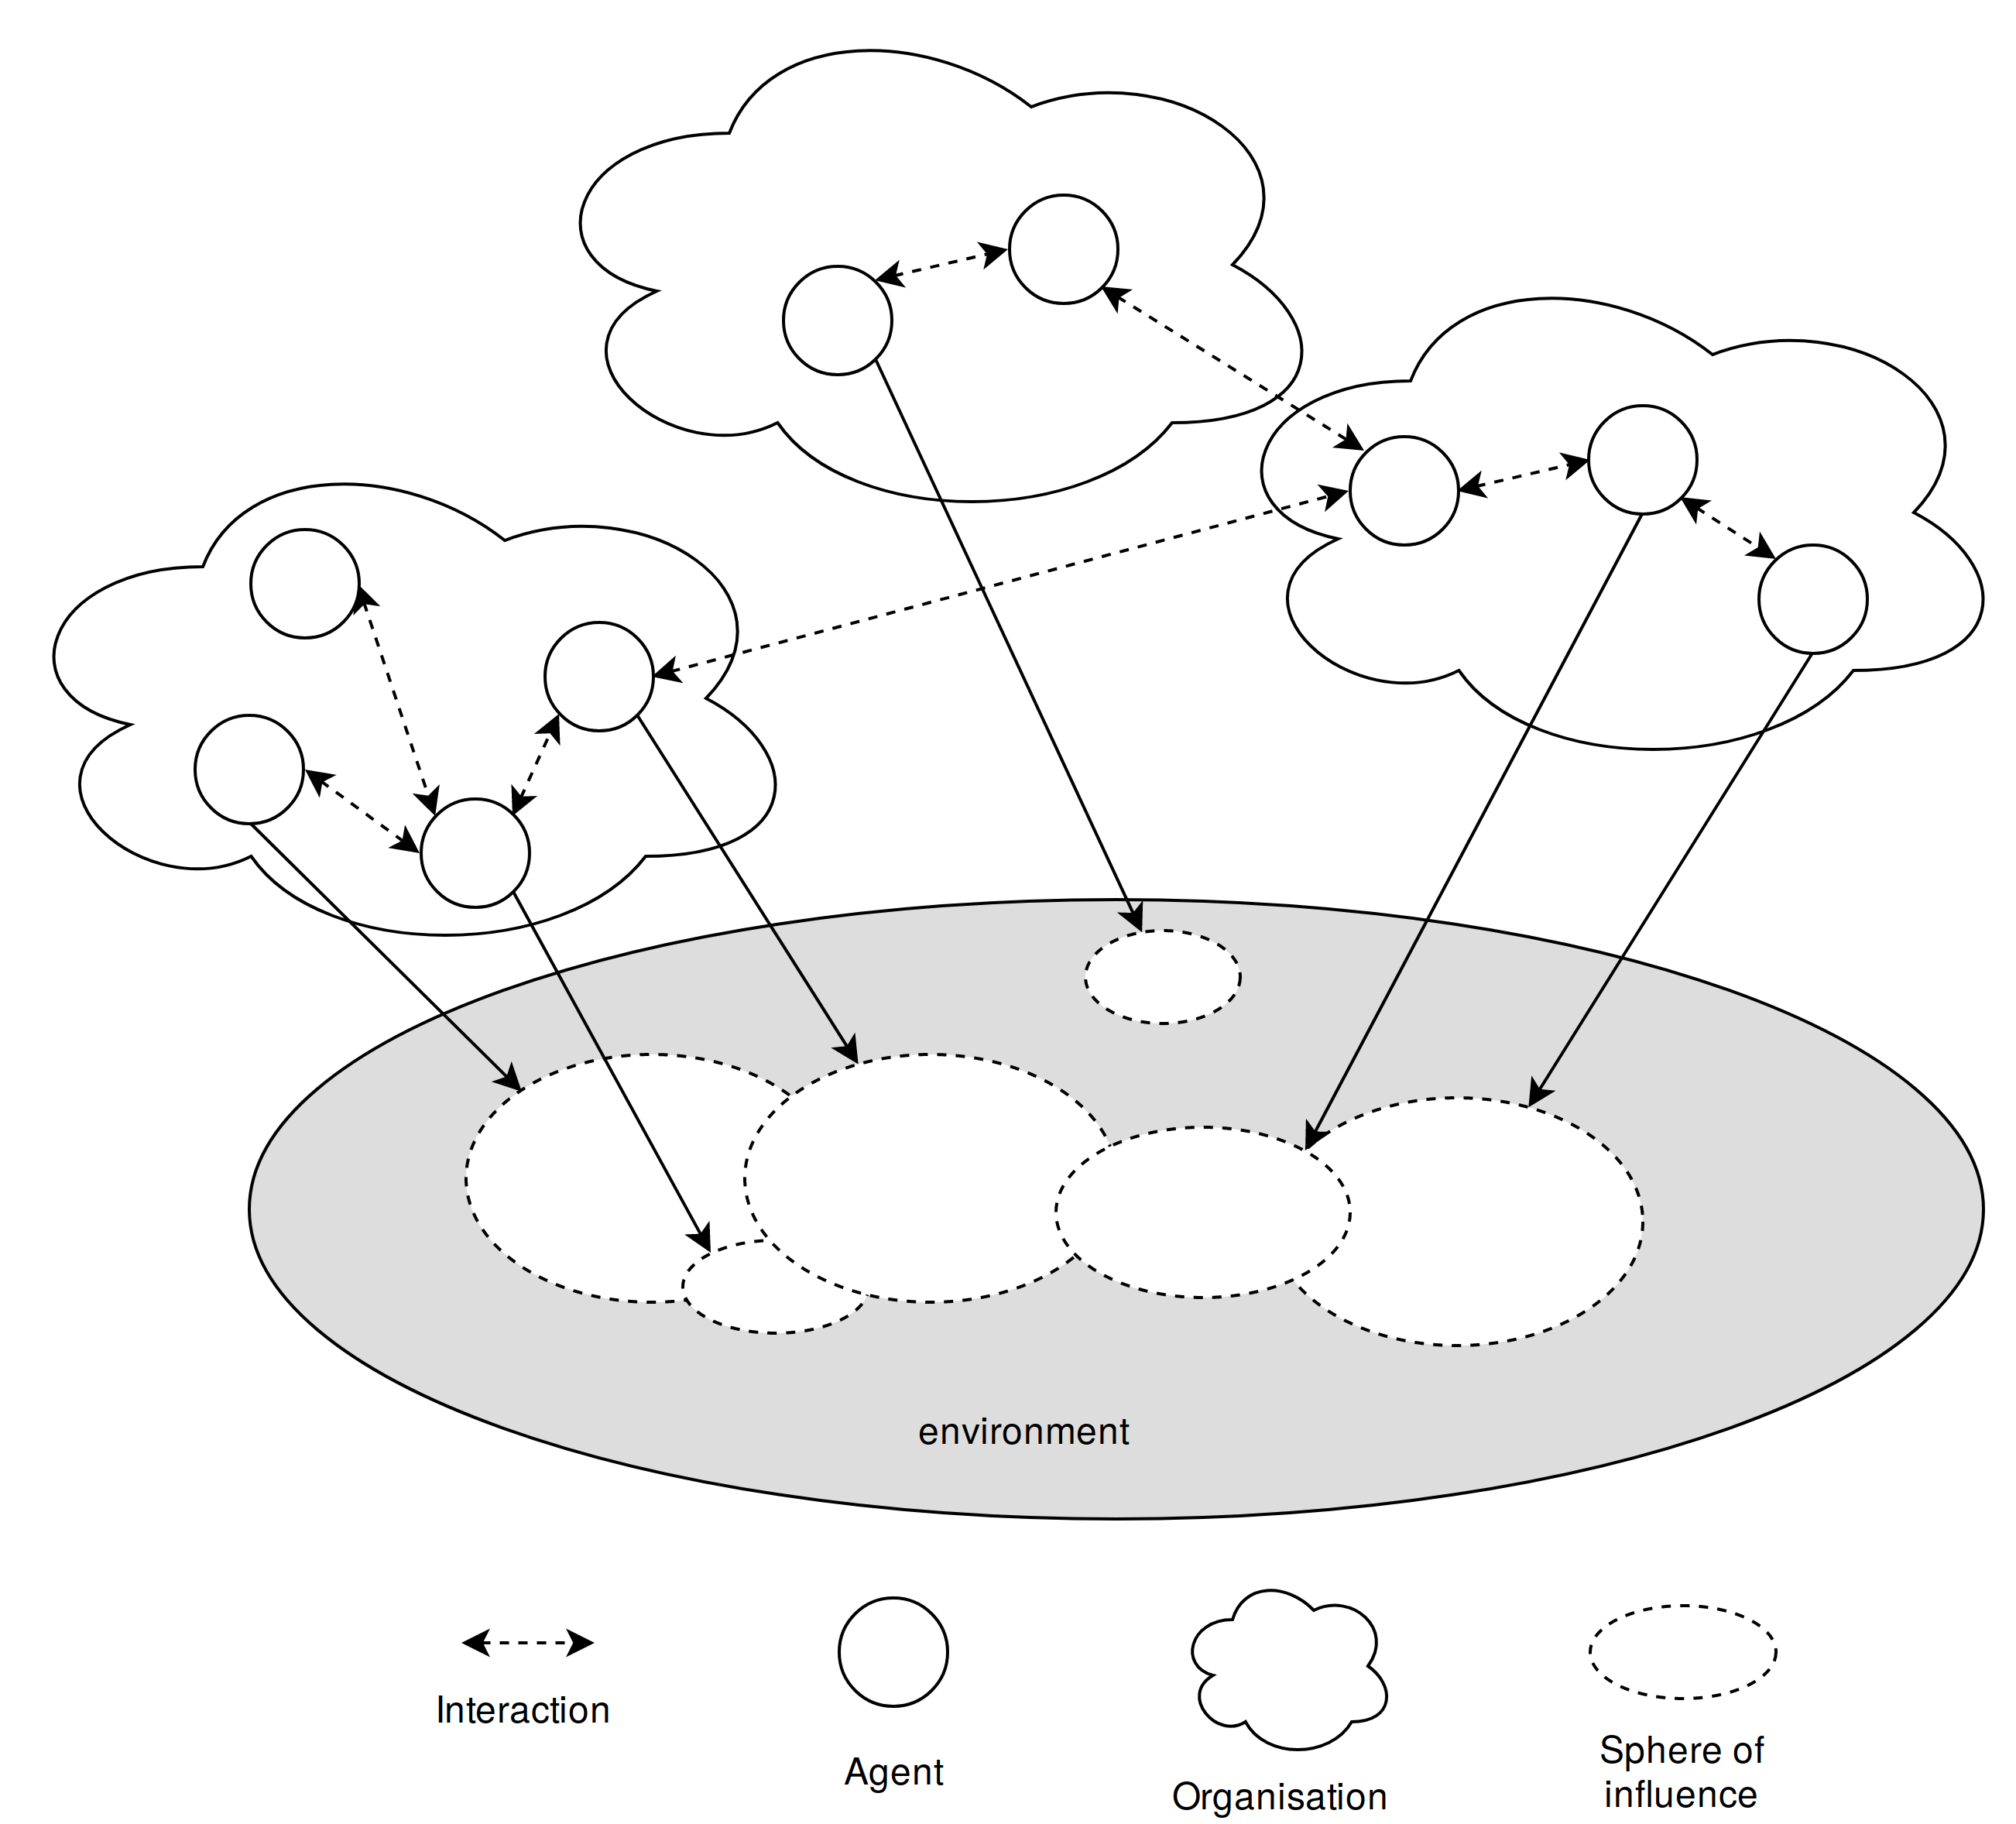
\includegraphics[width=\textwidth]{JenningsMAS.png}
	\caption{Jennings'~\cite{jennings2000agent} MAS conceptualisation}
	\label{fig:jenningsmas}
\end{framed}
\vspace{-30pt}
\end{wrapfigure}
When spheres of influences overlap an agent may need to make a decisions that is dependent upon other agents decisions. These overlaps can be described as interactions. Agents in these interactions are assumed to be self-interested, and want to improve their utility. Utility is the the representation of how beneficial events and actions in a system that transform the state of that system are to agents. Game-theoretic techniques can be used to model and simulate agent interactions using these utility functions. 

\section{Game Theory}
\label{sec:backgroundgametheory}
\subsection{Introduction}

\subsection{Cooperative Phenomena}
Game theory formulates mathematical models to study conflict and cooperation between intelligent rational decision-makers~\cite{myerson2013game}. In these mathematical models actions are often defined in terms of cooperation and defection. These models apply to more than just multi-agent interactions, including the natural world.\par 
Early evolutionary theory struggled to explain why cooperation is so prevalent in nature. In fact, it seemed that competition was key to evolution as individuals were competing to survive; the notion famously coined by Herbert Spencer ``Survival of the fittest''~\cite{spencer1864principles}.\par
Axelrod and Hamilton~\cite{evolution_of_cooperation} note two key areas of study that attempt to explain cooperative phenomena in the face of competitions: Kinship Theory and Reciprocal Altruism. These two theories are useful for explaining cooperation in nature, and as such, it may be possible to apply them to MASs in order to facilitate the evolution of cooperation between agents. Due to reasons explained in my appendix in subsection~\ref{appendix:kin} I will be focusing on reciprocal altruism.
\textcolor{red}{edit appendix entry to reflect this}

\subsection{Reciprocal Altruism}
\begin{wrapfigure}{l}{0.5\textwidth}
\vspace{-20pt}
\begin{framed}
	\center
	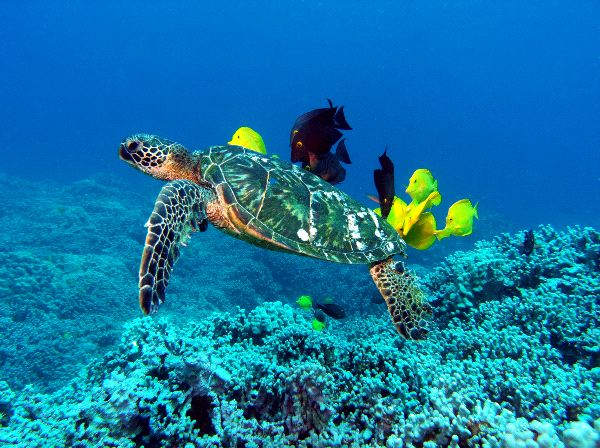
\includegraphics[width=\textwidth]{Green_Sea_Turtle_Cleaning_Station.jpg}
	\caption{Cleaning symbioses such as that of the green sea turtle and surgeonfish including the yellow tang show that reciprocal altruism is possible between non-humans and even interspecies~\cite{turtle}}
	\label{fig:cleaning}
\end{framed}
\vspace{-20pt}
\end{wrapfigure}
Reciprocal altruism is an idea most famously put forward by Robert L. Trivers~\cite{trivers1971evolution}. Trivers defines altruism as behaviour of one organism that benefits another to whom it is not closely related, while being apparently detrimental to the organism performing the behaviour. From this definition and from Trivers' description we can draw the meaning of reciprocal altruism to be altruism-based on the idea that the altruistic act will be returned.\par
This idea is a move away from limiting individuals to cooperating with only their kin - a key limitation of Kinship Theory - and towards any individual that they believe their cooperation will be reciprocated by. Axelrod and Hamilton~\cite{evolution_of_cooperation} noted this concept as advantageous in explaining cooperation between unrelated individuals, such as is common between humans. I would argue that this concept is also more applicable to higher intelligence societies such as those possible from MASs.

\subsection{Axelrod, Hamilton and The Iterated Prisoner's Dilemma}
\label{sec:ipd}
\begin{wrapfigure}{l}{0.4\textwidth}
\vspace{-20pt}
\begin{framed}
	\center
	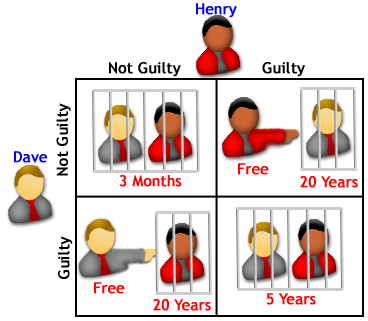
\includegraphics[width=\textwidth]{LaymansIPD.png}
	\caption{A fomulation of the Prisoner's Dilemma payoff matrix~\cite{laymansipd} similar to Rapoport \textit{et al.}~\cite{rapoport1965prisoner}}
	\label{fig:ipdvis}
\end{framed}
\vspace{-20pt}
\end{wrapfigure}
The prisoner's dilemma was described by Rapoport \textit{et al.}~\cite{rapoport1965prisoner} in terms of criminals under interrogation, but Axelrod and Hamilton formulated it in terms of cooperation and defection. This formulation allows the study of a more generic form of interaction betwenn individuals.\par 
In a single round of the prisoner's dilemma two individuals simultaneously choose to either cooperate or defect. After each interactions each individual receives a payoff in the form of a number, the higher the payoff the better. This payoff is dependent upon the actions of both individuals and is illustrated in table~\ref{tab:payoffmatrix}.\par
\begin{wrapfigure}{r}{0.6\textwidth}
\vspace{-20pt}
\begin{framed}
	\begin{center}
		\begin{tabular}{cc|c|c}
		& & \multicolumn{2}{c}{Player B}\\
		& & Cooperation & Defection\\
		\cline{1-4}
		\multirow{4}{*}{Player A} &\multirow{2}{*}{Cooperation} & A=3 & A=0\\
		& & B=3 & B=5\\
		\cline{2-4}
		& \multirow{2}{*}{Defection} & A=5 & A=1\\
		& & B=0 & A=1\\
		\end{tabular}
		\captionof{table}{The payoff matrix in a typical iterated prisoner's dilemma game (such as Axelrod and Hamilton's~\cite{evolution_of_cooperation}). A=x, B=y where x denotes the payoff for A and y denotes the payoff for B.}
		\label{tab:payoffmatrix}
	\end{center}	
\end{framed}
\vspace{-20pt}
\end{wrapfigure}
From an agents perspective we can view the payoff in terms of utility or what is preferable to an agent~\cite{wooldridge2009introduction}. Using player A and player B, with $u_i$ being the utility function for agent i, and the payoff matrix provided by Axelrod and Hamilton~\cite{evolution_of_cooperation} we have the following utility functions: $u_A(D,D)=1$, $u_A(D,C)=5$, $u_A(C,D)=0$, $u_A(C,C)=3$ for player A and $u_B(D,D)=1$, $u_B(D,C)=0$, $u_B(C,D)=5$, $u_B(C,C)=3$ for player B.\par 
We can order the possible situations by utility for each agent to understand what situations are preferable to each agent. For player A: $(D,C)\ge (C,C)\ge (D,D)\ge (C,D)$. For player B: $(C,D)\ge (C,C)\ge (D,D)\ge (D,C)$. As you can see players are at odds as to which situations they wish to arise. If both attempt to bring about the situation that is preferable to them they will both receive only $1$ as payoff each.\par 
In the iterated prisoner's dilemma the two agents repeat these rounds and can base their decisions on previous rounds. This allows individuals to use strategies that make use of a mechanism known as direct reciprocity~\cite{five_rules_coop}, which is a type of reciprocal altruism.\par 
Axelrod and Hamilton~\cite{evolution_of_cooperation} used games of the iterated prisoner's dilemma in their round-robin tournaments. These tournaments had a set of players that are associated with strategies. Every player entered into a game against every other player, in which rounds were repeated. For cooperation to be rational in the iterated prisoner's dilemma the `shadow of the future' needs to present in each round~\cite{wooldridge2009introduction}, so games were not cut off at a set point but ended by increasing the probability the game won't continue each round.\par 
Axelrod and Hamilton~\cite{evolution_of_cooperation} combined these round robin tournaments with a genetic algorithm~\cite{mitchell1998introduction} (genetic algorithms are discussed in subsection~\ref{subs:backgroundreproduction}). One aim of Axelrod and Hamilton's~\cite{evolution_of_cooperation} paper was to review how successful the strategies submitted to them were. The use of a genetic algorithm allowed them to ask three questions of each strategy. Is it robust? Is it stable? Is it initially viable?\par
Robustness refers to the ability to thrive in an environment with a variety of strategies. Stability refers to the ability to - once fully established - resist invasion by mutant strategies. Initial viability refers to whether or not a strategy can establish itself in a non-cooperative environment.\par
Axelrod and Hamilton~\cite{evolution_of_cooperation} found two strategies with these three abilities: 'tit-for-tat' and 'all defect'. Later on, Nowak and Sigmund~\cite{nowak-1993a} found that 'Pavlov' ('win-stay, lose-shift') also has these abilities. The interesting part of 'Pavlov' and tit-for-tat is that they are nice strategies (they begin by cooperating) and that they also actively aid in the evolution of cooperation.\par
Nowak~\cite{five_rules_coop} found that for the evolution of cooperation to occur, the cost-to-benefit ratio of the altruistic act must be less than the probability of another encounter for cooperation to evolve: $w>c/b$. If the probability of subsequent encounters between two individuals is low, then it is very likely that cooperation will not evolve as there will be no sufficient reward. With the advent of huge networks spanning across the world and the drastic increase in devices across these networks, it is highly likely MASs will operate with IAs that are unlikely to re-meet.\par
Axelrod and Hamilton's program was not created as a MAS. However, the importance of remeeting is a definite limitation to the use of direct reciprocity in MASs, and as such I do not see direct reciprocity as a strong contender to encourage cooperation on its own. One required property of a mechanism to encourage cooperation is that it must work when both re-meeting is unlikely and when it is likely. As such, direct reciprocity is not completely inadequate for the problem. However, it is insufficient when not combined with some encouragement for when chances of meeting again are low.\par
Extensive interest in reciprocal altruism in recent years has been focused towards direct reciprocity, including a number of available libraries such as the Axelrod Python library~\cite{axelrodproject}. I argue that to gain a better understanding of how we can work to facilitate cooperation between IAs, we must look at a wider berth of options.

\subsection{Indirect Reciprocity}
\begin{wrapfigure}{l}{0.5\textwidth}
\vspace{-20pt}
\begin{framed}
	\center
	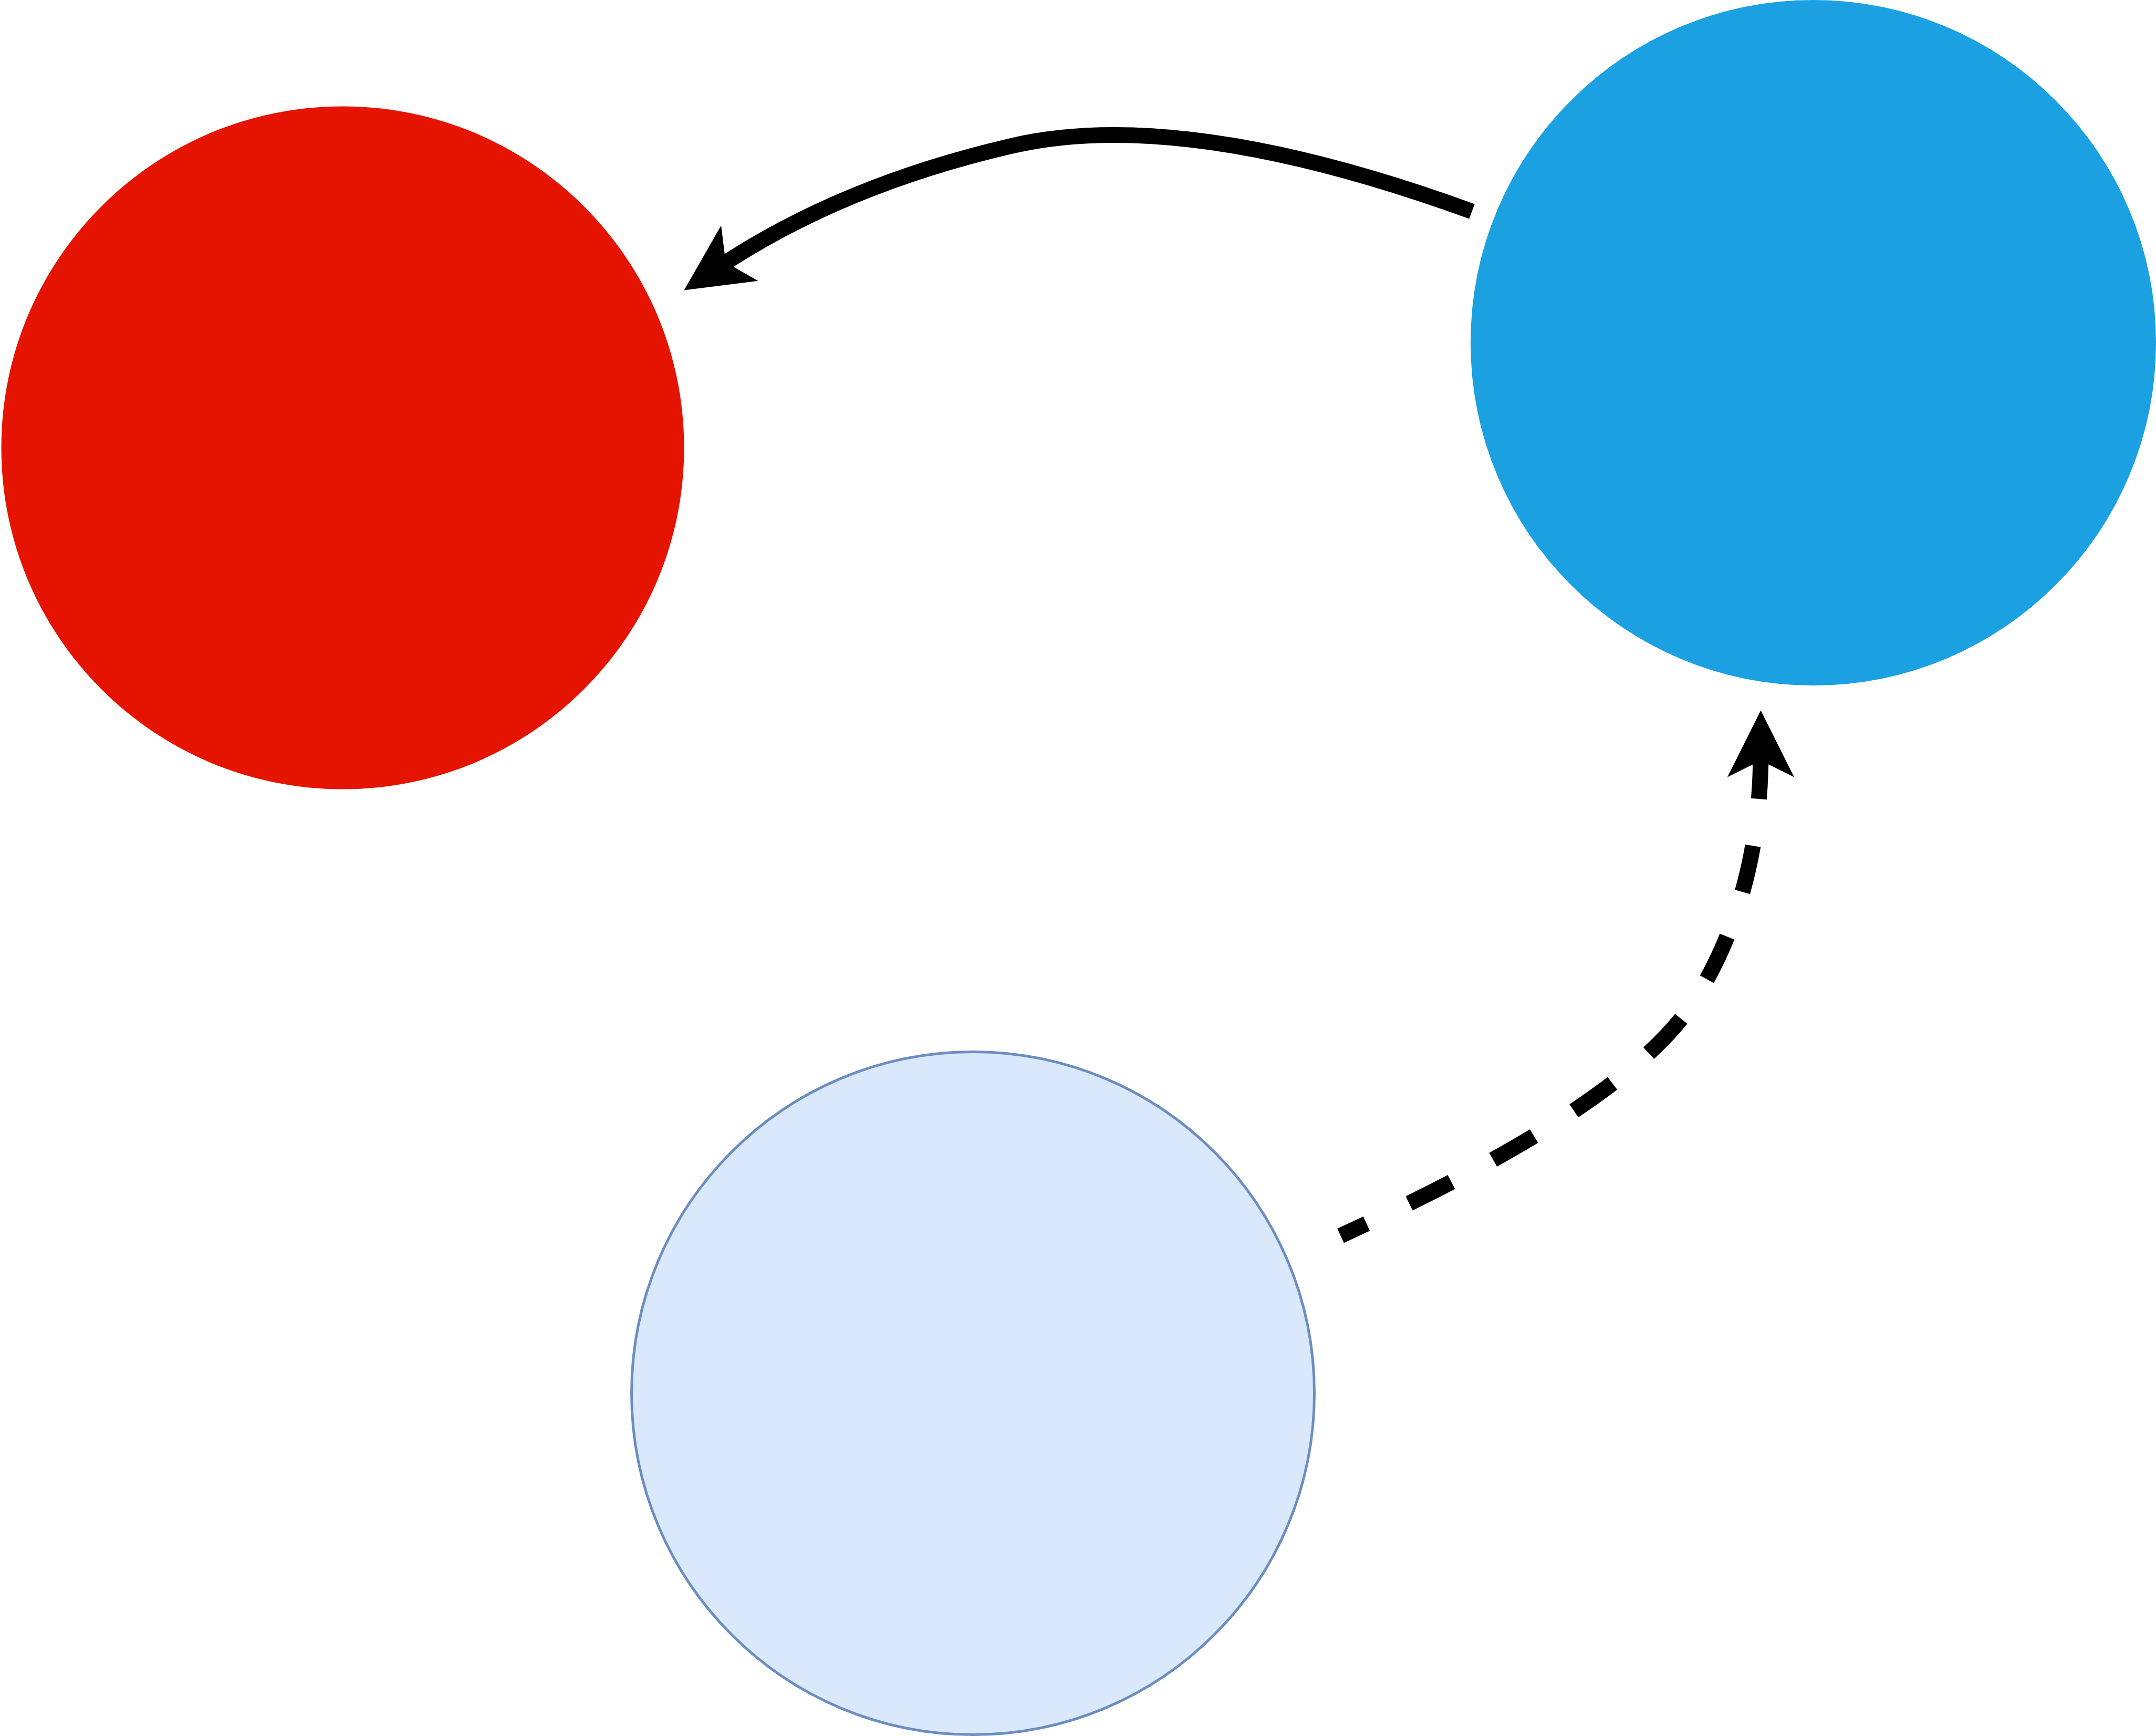
\includegraphics[width=\textwidth]{IndirectRec.png}
	\caption{The main idea of indirect reciprocity from Nowak~\cite{five_rules_coop}}
	\label{fig:indir_rec}
\end{framed}
\vspace{-20pt}
\end{wrapfigure}
Nowak~\cite{five_rules_coop} presents five mechanisms that aim to facilitate the evolution of cooperation. Direct reciprocity is used in the iterated prisoner's dilemma. I discuss three others in my appendix (subsections~\ref{appendix:kin, appendix:groupselection, appendix:netreciprocity}) and the final one I shall discuss here: indirect reciprocity\par
This concept is promising for use in MASs as it solves the failure of direct reciprocity's failure with regards to when re-meeting is low. In a large society or a vast network in which agents are likely to operate in success when re-meeting is low is an important property. We will see later on that the two mechanisms can be combined.\par
Indirect reciprocity uses the group mechanic of reputation to encourage cooperation. Alexander~\cite{alexander1987biology}, who was an early advocate the idea, focused on human reciprocal altruism, however, subsequent research has abstracted away from the biology~\cite{phelps_game_theoretic_analysis, imagevsstanding, evol_indirect_image, evoldirindir, five_rules_coop, leimarhammer, sugden2004economics, gossip_alt, mui2002computational}. The idea is that if an individual cooperates with another individual, then their reputation will be enhanced in the community. This boost of reputation makes it more likely that they will be helped by others later on. Thus this mechanism a form of reciprocal altruism.\par
According to Nowak and Sigmund~\cite{evol_indirect_image} the reputation mechanic requires a higher level of intelligence than direct reciprocity, due to the complexity of group mechanics in the system. It is this kind of higher level intelligence which is required to reason about events in a group that could be a key part in the development of MASs.\par
Due to this reason, I feel that either indirect reciprocity or possibly a combination of both direct and indirect reciprocity is a good candidate for a mechanism to study further. For the rest of this literature review I will consider both past approaches to indirect reciprocity and other factors in the mechanism that can be used to facilitate the evolution of cooperation.


\subsection{Nowak and Sigmund}
\label{sec:nowak_sig}
According to Gilbert Roberts~\cite{evoldirindir}, Nowak and Sigmund~\cite{evol_indirect_image} is the most influential model on indirect reciprocity. Therefore, I shall examine this model of indirect reciprocity first. Nowak and Sigmund begin by stipulating that human cooperation is due to people's `image' of each other, which is comparable to reputation. Nowak and Sigmund converted the image to an integer score between -5 and 5 for simplicity.\par
The idea is simple, cooperation increases your image score by 1 and defection reduces it by 1. The higher your image score the more likely it is you will receive help. Nowak and Sigmund claim that this mechanism channels cooperation toward valuable members of the society of players.\par
Nowak and Sigmund note that the use of image scores and indirect reciprocity itself, leave a system open to anticipation, planning, deception and manipulation. These 4 concepts seem closely related to possible happenings in MASs. Deception and manipulation are two factors that I think are worth experimenting with. At the same time, anticipation and planning are a key part of agent design in multiple languages and frameworks. In fact the lack of planning was such an important drawback of the Agent0 language~\cite{shoham1991agent0} Becky Thomas created a new language - PLACA~\cite{thomas1993placa} - which allowed agents to plan, among other improvements.\par
The framework created by Nowak and Sigmund is simplified from Alexander's~\cite{alexander1987biology} idea of human reciprocal altruism. Nowak and Sigmund describe a framework in which there is a population of individuals which act as a pool to select pairs in which one player is the donor - who can choose whether to cooperate or defect - and the other is the recipient of this action. A cooperation costs the donor $c$ to its fitness and benefits the recipient's fitness the value of $b$ where $b>c$. Whereas a defection costs nothing and the recipient is not benefitted. This is shown in the payoff matrix in table~\ref{tab:indirrec_payoffmatrix}.\par
\begin{wrapfigure}{l}{0.5\textwidth}
\vspace{-20pt}
\begin{framed}
	\begin{center}
		\begin{tabular}{c|c|c}
		\multirow{2}{*}{Donor Action} & \multicolumn{2}{c}{Payoffs}\\	
		& Donor & Recipient\\
		\hline
		Cooperation & -1 & 2\\
		\hline
		Defection & 0 & 0\\
		\end{tabular}
		\captionof{table}{The payoff for Nowak and Sigmund's~\cite{evolution_of_cooperation} indirect reciprocity model}
		\label{tab:indirrec_payoffmatrix}
	\end{center}	
\end{framed}
\vspace{-20pt}
\end{wrapfigure}
As noted above, these actions also affect the donor's image score, but Nowak and Sigmund add a caveat when using the idea of onlookers. The notion of onlookers limits the visibility of actions in the society by randomly selecting a group of specified size to view each interaction. This concept is displayed graphically in figure~\ref{fig:onlookers}. The concept of onlookers was added due to the realisation of Nowak and Sigmund's that in a group that is spread over a wide geographical area, not all individuals will be able to view each interaction. This sparse nature of interactions is of course especially likely in MASs. Image scores now become one player's view of another rather than a community view of the player. A matrix $ImageScore$ is used to store these scores.\par
The discriminator is the strategy of choice for Nowak and Sigmund. This strategy stores a number $k$, and when the individual $u$ using that strategy is a donor to the individual $v$, $u$ cooperates if the value $ImageScore[u,v]>=k$ otherwise it defects~\ref{fig:image_discriminator}. This strategy is incredibly simple yet effective. The model also includes the defector and cooperator strategies. Nowak and Sigmund detailed more strategies. These strategies base their decisions not only on that of the recipient's image score but also their own. In this way, the individual will be able to decide whether it is important to boost their reputation in the system in order to receive cooperation or not.\par
Similarly to Axelrod and Hamilton's tournaments~\cite{evolution_of_cooperation} Nowak and Sigmund~\cite{evol_indirect_image} used a genetic algorithm to find optimal strategies under certain conditions. They varied conditions such as the length of each generation and the number of onlookers per interaction.\par 
Nowak and Sigmund hypothesize and give evidence supporting the idea that the length of the generation is important to the evolution of cooperation. They highlight that when $m$ donor-recipient pairs are selected in succession in a population of size $n$, a player is likely to be selected as part of a pair $2m/n$ times. According to their evidence, the higher this value of $2m/n$, the more likely cooperation will evolve.\par
Another idea put forward and evidenced by Nowak and Sigmund is that the evolution of cooperation is dependent upon the donor's knowledge of the image score of the recipient. This chance of knowing an image score is limited by the concept of onlookers. However, in Nowak's 2005 paper on the five rules of cooperation~\cite{five_rules_coop} he talks about using `gossip' as an alternative to direct observation. Gossip and social ability are interesting concepts in MASs. According to Wooldridge and Jennings~\cite{wooldridge_jennings_1995}, social ability is a key property in even a weak notion agents.\par
The model laid out by Nowak and Sigmund is succinct and a good basis for looking at interactions in multi-agent systems. Similarly to Axelrod and Hamilton~\cite{evolution_of_cooperation} Nowak and Sigmund~\cite{evol_indirect_image} did not create a MAS to run their games.\par
If they had been considering MASs they may have noticed a number of limitations. The first limitation I will highlight is the way in which reputation is implemented. In the version without onlookers each player has a global image score and even in the version with onlookers there is a public matrix encoding all image scores.\par
Image scores could be seen as a community view of an individual. However, I argue that the idea that image scores are attempting to capture (reputation) is actually more personal. Although there might be a rough consensus as to an individual's general reputation among people in a society, this reputation is often conveyed through social means and is subject to the personal interpretation of each individual.\par
According to Russell and Norvig~\cite{russell2016artificial}, IAs use an internal state. It is in this internal state, I argue, that image scores should be stored in order for an agent to have full control over them. Trust models could be devised to manage these image scores. This idea is a closer match to the MAS paradigm and it would allow for a truly distributed system.\par
Indirect reciprocity makes a good candidate for use in MASs and this model is both very influential and a good basis for those MASs. The model includes extensive interesting aspects that have been examined carefully including the onlookers and reproduction mechanisms, and also includes ideas that have not been fully researched such as a gossip systems and using deception and manipulation to affect the system. These features allow more room for me to explore if I use Nowak and Sigmund's model as a basis, with a few alterations to more closely match the MAS paradigm.
\begin{figure}
	\center
	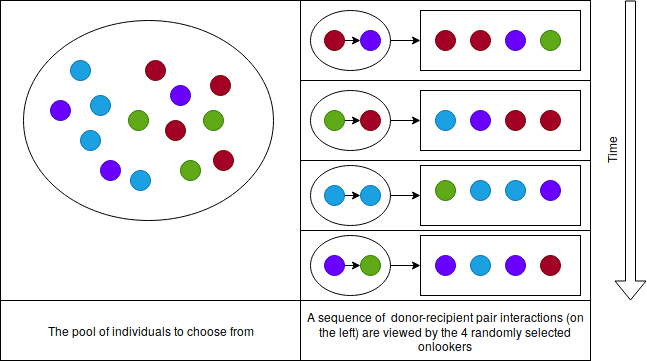
\includegraphics[width=0.7\textwidth]{Onlookers.png}
	\caption{The selection of a sequence of donor-recipient pairs and onlookers in Nowak and Sigmund's~\cite{evol_indirect_image} model of indirect reciprocity. The macro-view of indirect reciprocity. The lines and arrows show the spread of information.}
	\label{fig:onlookers}
\end{figure}
\begin{figure}
	\center
	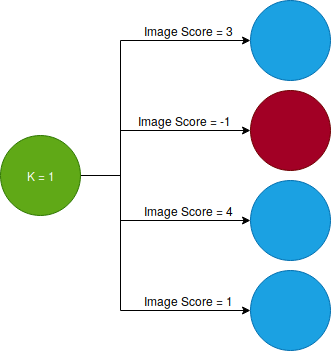
\includegraphics[width=0.3\textwidth]{Image_Scoring.png}
	\caption{On the left an image scoring discriminator with K=1. On the right the agents the discriminator is a donor for. Blue agents represent where there would be a cooperation from the donor, red represents when the discriminator would defect against them. The rule is when $Image Score >= K$ cooperate else defect.}
	\label{fig:image_discriminator}
\end{figure}

\subsection{The Standing Strategy and Further Limitations of Nowak and Sigmund}
Leimar and Hammerstein~\cite{leimarhammer} criticised Nowak and Sigmund's~\cite{evol_indirect_image} limited range of strategies. They also highlighted the abilities of another strategy, the standing strategy, over image scores.  The standing strategy was first described by Sugden~\cite{sugden2004economics} and and uses a `switch'~\cite{evol_indirect_image}.\par
Milinski \textit{et. al}~\cite{imagevsstanding} described the standing strategy as the idea that an individual does not only aim for a good fitness but also a good standing. Each individual holds other individuals in either a good or bad standing, which starts out as good until perceived otherwise. The event that causes the switch from good to bad is an individual defecting against another with a perceived good standing.\par
The idea is that it is morally incorrect to defect against a good individual, but defecting against a bad individual is acceptable as it punishes those members of society that are not valuable. There is conflict between the use of image scores and the standing strategy.\par
The argument for the standing strategy is as follows: When using image scoring, if a discriminator has $k=0$ and is a donor to another with an image score of $-1$, they will defect. This action is seen as punishing a bad individual, as it channels fitness away from bad members of the society. However, the donor's image score is reduced by 1. This change in score decreases the chance that the donor will receive cooperation from others, so there is no real incentive for them to punish the bad members of that society, except for pure altruism.\par
Conversely, the standing strategy only reduces the reputation of those who defect against good individuals. Therefore, punishing bad members of the society has no negative effect on those members. Leimar and Hammerstein~\cite{leimarhammer} argue that Sugden's version of indirect reciprocity and his use of the standing strategy are more robust than Nowak and Sigmund's image scoring.\par
Milinski \textit{et. al}~\cite{imagevsstanding} analysed Leimar and Hammerstein's argument, suggesting that they were correct under conditions which allowed for perfect perception of events and unlimited memory capacity. However these conditions are not always true, especially in a MAS in which the environment is inaccessible~\cite{russell2016artificial}.\par
Nowak and Sigmund claimed that indirect reciprocity is open to deception and manipulation, especially when we consider the use of gossip in a system. Gossip opens IAs to imperfect perception of other IAs. Therefore, it would be interesting to see which strategy is more effective in a system in which other IAs actively attempt to deceive using gossip, and the information received is not always perfect.

\subsection{Mixed Reciprocity Models}
Roberts~\cite{evoldirindir} and Phelps~\cite{phelps_game_theoretic_analysis} noted that indirect reciprocity is focused towards interactions with other individuals with whom the donor has no previous interactions. However, what about when re-meeting is more likely? I stipulate that an individual is affected by both being the recipient of actions and their observation of actions. Roberts engaged with the issue by introducing an experience score. This experience score works similarly to an image score but is bounded by -1 and 1. It increases when the individual is a recipient of a cooperation, and decreases when receiving a defection.\par
Roberts also created a version of the standing strategy which uses an image score (-1 to 1). However herein, the value changes according to the rules of the standing strategy rather than Nowak and Sigmund's rules.\par
Both Roberts and Phelps measured the use of indirect reciprocity against the use of direct reciprocity. Roberts concludes that indirect reciprocity is the more popular decision mode under conditions in which re-meeting was less common, and direct was more popular when re-meeting was frequent. On the other hand, Phelps' experiments garnered different results being that in small groups direct and indirect reciprocity exist in equilibrium.\par
Similarly to Nowak and Sigmund~\cite{evol_indirect_image}, Roberts I believe falls short in recognising how personal interpretation of events are. There are many different trust models a player could use by mixing interpretation of events in which they are the recipient and also in which they are not the recipient. For example, it could be expected that being on the receiving end of a defection means that a player is likely to be more hardline, than when they observe a defection against another. However, Roberts limits the study to using a simple experience score.\par
I would suggest using a model similar to that I described in section~\ref{sec:nowak_sig}, in which interpretation of events is up to an agents trust model. Some trust models could interpret events when the agent is the recipient different to those in which they are observing.

\subsection{Gossip}
Nowak and Sigmund~\cite{evol_indirect_image} realised the issues surrounding the fact that all individuals being able to view interactions in their simulation framework is not concomitant with real life. As such, they introduced the idea of onlookers as noted in section~\ref{sec:nowak_sig}. An issue with limiting observation is that knowing an accurate image score of a player is important to the evolution of cooperation in an indirect reciprocity system. Nowak~\cite{five_rules_coop} suggested using gossip to spread information regarding image scores in their simulation framework.\par
Sommerfeld \textit{et al.}~\cite{gossip_alt} conducted an empirical study on gossip between cooperative and uncooperative individuals in an indirect reciprocity setup. The experiment consisted of humans playing a number of indirect reciprocity rounds to build up a cooperation history, and then a smaller number of gossip rounds. These rounds were then repeated to see how the individuals reacted to the gossip.\par
The focus of the experiment was to look at gossip composition, gossip transfer and resulting behaviour. The findings included that gossip is an effective method of spreading reputation information in an indirect reciprocity system, on fulfilment of some conditions, the first of which is the truthfulness of the gossip. Gossip must accurately reflect the behaviour of the subject of the gossip.\par
Another condition is the comprehensibility of the gossip. The language used in the gossip must be interpretable by the recipient of the gossip. In an agent system this condition would require an agent communication language (ACL) (such as KQML~\cite{finin1994kqml} or FIPA-ACL~\cite{o1998fipa}) and would also require the content of the messages that use this language to be interpretable by the recipient agent. The final condition is that individuals must act accordingly based on the gossip they receive.\par
These three conditions of a system would have to be created by building strategies for agents that attempt to uphold them, and a communication language to support accurate and interpretable information. Nowak and Sigmund~\cite{evol_indirect_image} identified that indirect reciprocity systems can be effected by deception and manipulation from malicious players. The addition of gossip creates a meta-game on top of the indirect reciprocity system. Players must have a trust model that differentiates between dealing with gossip and with directly observed interactions, and a strategy on spreading gossip effectively.
\begin{figure}
	\center
	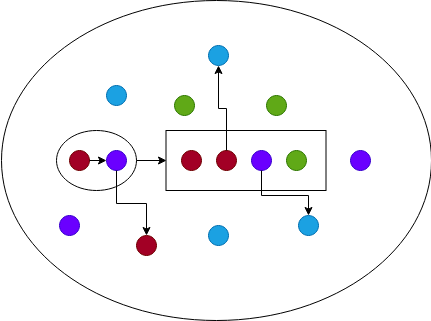
\includegraphics[width=0.5\textwidth]{Gossip_and_onlookers.png}
	\caption{The spread of information (shown through the lines) through a population using indirect reciprocity with gossip and onlookers}
	\label{fig:gossip_and_onlookers}
\end{figure}

\subsection{Mui's Computational Models of Trust and Reputation}
Mui~\cite{mui2002computational} presented an indirect reciprocity simulation framework similar to Nowak and Sigmund~\cite{evol_indirect_image} that spreads social information through `acquaintance networks' to inform a donor's decision. An individual in this framework builds up a network of players whom they meet through interaction, their `acquaintance network'. If this individual is then a donor in a donor-recipient pairing the individual consults their acquaintance network regarding the recipient. The information gathered from this network helps a donor to decide if they can trust the recipient to reciprocate their cooperation; known as `collective memory'.\par
Baumeister \textit{et al.}~\cite{baumeister2004gossip} advocated for the idea that gossip is used for four functions, including strengthening bonds between the gossiper and recipient, enabling the spread of information about the subject (one function for each positive and negative reasons), and helping to educate individuals about the complex cultural systems they reside in.\par
I would argue that indirect reciprocity systems and MASs are complex cultural systems in which gossip can be applied for these four functions. Mui's acquaintance networks support this gossip functionality to a certain extent; however they are limited by the lack of proactivity of gossip. Sommerfeld \textit{et al.}~\cite{gossip_alt} highlighted the willingness of their participants to spread gossip, and the last function of gossip proposed by Baumeister \textit{et al.}~\cite{baumeister2004gossip} (cultural education) suggests that for gossip to be most effective the gossip should be proactively spread.\par
As a result, I believe that a theoretical framework which uses gossip should allow a proactive social ability  by using gossip as an action at times at which an agent is not acting as a donor. 

\subsection{Reproduction and Genetic Algorithms}
\label{subs:backgroundreproduction}
As discussed in section~\ref{subs:env} finding the best solution from a set of possible solutions is an optimisation problem. Genetic algorithms are an approach to solve optimisation problems, and as such my system will be acting like a genetic algorithm with simulate reproduction.\par
Between each generation a reproduction phase occurs, in which agents are created and associated with strategies for the next generation. Nowak and Sigmund~\cite{evol_indirect_image} and Axelrod and Hamilton~\cite{evolution_of_cooperation} (though indirectly their payoff scores do seem to equate to fitness) used a reproduction mechanism inspired by Herbert Spencer's~\cite{spencer1864principles} famous phrase ``Survival of the fittest''.\par
Wooldridge's~\cite{wooldridge2009introduction} argument that agents attempt to fulfil a design objective using their own autonomy suggests that strategies for agents will only be used in practice if they are successful in their design objective. The main design objective of players in my game is to interact with players to increase their fitness, with some having other big objectives such as aiding in the evolution of cooperation.\par
The measurement of how successful an agent is in my system is thus their fitness score. Just like in Nowak and Sigmund's, and Axelrod and Hamilton's reproduction mechanism I propose using a ``Survival of the fittest approach''. The real replicated information in my system is the strategy an agent uses, so the mechanism I am using makes it more likely for strategies with higher overall fitness scores across agents in a generation to be reproduced.\par
Francq~\cite{genetic_algorithms} puts forward two types of reproduction: proportional selection and tournament selection.\par
Proportional selection translated to my system and simplified would look something like the following. Take a roulette with p (number of players) slots and divide the p slots into n (number of strategies) sections. The size of each section is directly proportionate to the average fitness of all players of a certain strategy. For example strategy A has 2 agents with fitness 4 and 6 respectively, strategy B has 4 agents with fitness 3, 8, 9 and 4 fitness respectively and strategy C has 1 agent with fitness 7. The average fitness of A is 5, B is 6 and C is 7, so A would receive 5 slots of the roulette wheel, B 6 slots and C 7 slots. The resulting roulette wheel displayed in~\ref{fig:roulette_wheel} is spun and a ball dropped and whichever slot the ball landed on the corresponding strategy is selected for the new player.\par
\begin{figure}
	\begin{center}
	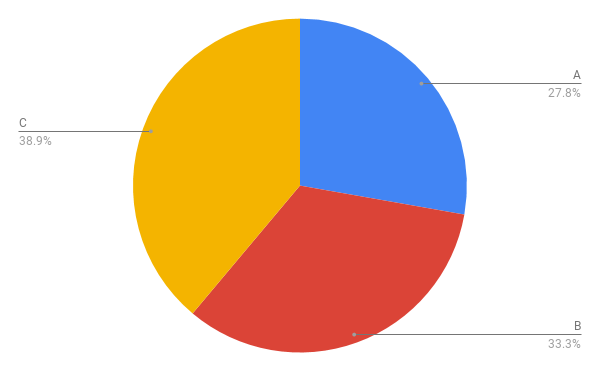
\includegraphics[width=0.5\textwidth]{reproduction_chart.png}
	\caption{The roulette wheel from my proportional selection example}
	\label{fig:roulette_wheel}
	\end{center}
\end{figure}
Tournament selection could be translated in the following way. Have an empty list which will contain an ordered list of agents. In a loop (until the population is of size 1): select two agents from the population, remove the lowest fitness one and insert it into the list. After the loop insert the last agent into the top of the list. The top of the list always contains the highest fitness agent. Using the same population of agents in the proportional selection algorithm we can give an example of this in table~\ref{tab:tournament_selection}.
\begin{framed}
	\begin{center}
		\begin{tabular}{c|c|c|c}
		Set & Test & Put in List & List\\
		\hline
		${A_1, A_2, B_1, B_2, B_3, B_4, C_1}$ & $(A_1, B_3)$ & $A_1$ & ${A_1}$ \\
		${A_2, B_2, B_3, B_4, C_1}$ & $(B_1, C_1)$ & $B_1$ & ${A_1, B_1}$\\
		${B_2, B_3, B_4, C_1}$ & $(A_2, C_1)$ & $A_2$ & ${A_1, B_1, A_2}$\\
		${B_2, B_3, C_1}$ & $(B_4, C_1)$ & $B_4$ & ${A_1, B_1, A_2, B_4}$\\
		${B_3, C_1}$ & $(B_2, B_3)$ & $B_2$ & ${A_1, B_1, A_2, B_4, B_2}$\\
		${B_3}$ & $(B_3, C_1)$ & $C_1$ & ${A_1, B_1, A_2, B_4, B_2, C_1}$\\
		$\emptyset$	& & $B_3$ & ${A_1, B_1, A_2, B_4, B_2, C_1, B_3}$
		\end{tabular}
		\captionof{table}{The payoff for my indirect reciprocity model}
		\label{tab:tournament_selection}
	\end{center}	
\end{framed}
Fitness proportionate selection seems to translate best to my system as there is an obvious and simple way to select each agents strategy for the new generation using the roulette wheel, unlike the tournament selection process which requires the crossover step. The crossover step requires a chromosome represented as a bit array to produce an offspring from two parents. This is analogous to sexual reproduction, but not the building of new agents.\par
Lipowski \textit{et al.}~\cite{lipowski2012roulette} presented an efficient version of roulette wheel selection using stochastic acceptance rather than the searching method used by Francq~\cite{genetic_algorithms}. The stochastic acceptance algorithm works like this: select randomly one of the individuals from the last generations population, with fitness of the individual as $w_i$ and $w_{max}$ the maximal fitness of the generation use the probability $w_i / w_{max}$ to select whether or not to use this agents strategy for a new generation agent, if not repeat. Lipowski \textit{et al.} proved mathematically that the probability distribution of this method and general roulette wheel selection are the same, and that the stochastic acceptance algorithm is more efficient as well.

\subsection{Summary}

\chapter{Framework}

\section{Introduction}
In the following sections of this chapter I will be discussing the theoretical side of my framework and the subsequent practical implementation of this framework.

\section{Theoretical Framework}
\label{sec:theo}

\subsection{Introduction}
In this section on the theoretical framework I will be presenting an overall design for my mixed reciprocity model and MAS. I have taken inspiration from past work on game theory (discussed in section~\ref{sec:backgroundgametheory}) and techniques for the development of MASs (from section~\ref{sec:backgroundmas}). Franklin and Graesser~\cite{franklin1996agent} stipulated that to describe an agent one must describe five aspects: the environment the agent resides in, the agent's sensing capabilities, the possible actions the agent can take, the drives or primative motivators for an agent's actions and the action selection architecture for the agent. I shall describe these five aspects in the following subsections here.

\subsection{The Game and Environment}
\label{subs:env}
The environment in which the agents will reside in my system will provide facilities for interaction between the agents. An instance of the environment in my system will be known as a generation. Each generation contains a set of agents. These sets of agents will act as pools to select donor-recipient pairs and onlookers for those pairs.\par
A generation is contained within a community. These communities contain multiple generations with a strict ordering. A game has distinct timepoints. The number of these timepoints vary according to the number and length of generations - which are variables set by the user at the start. Say these timepoints range from $1..n$ and there are generations $1..k$ where $k<n$ and $n\%k=0$. Then the timepoints are distributed evenly across each generation like this: \par \centerline{$\{\{1, .., (n/k)\},\ \{(n/k+1), .., (2n/k)\},\ ..,\ \{(n-(n/k)+1), .., n\}\}$}
\par 
The environment will work using a cycle in which each step follows the process perceive-decide-execute. Each step of the cycle is a timepoint. The perceive section of a step refers to when all agents receive perceptions generated for that timepoint - mostly from actions in the previous timepoint. All agents then decide on an action and the last part of the step is the execution of these actions in the environment.\par
The key to the cycle steps is that all agents perceive, after which all agents decide and then all actions are executed. The effect is to synchronise agents steps and prevent actions from a timepoint affecting other agents decisions at the same timepoint. Synchronicity keeps the environment static for the period in which an agent is deciding.\par
In each timepoint there is exactly one donor-recipient pair selected at random from the generation's pool of players. For that pair there is a group of onlookers, again randomly selected from the remaining players in the generation's pool.\par
As discussed, each generation contains a set of players which participate in the cycle steps for each timepoint of that generation. But how are these sets of players selected? For the first generation, a number of agents and associated strategies (subsection~\ref{subs:stratstrustmodels}) are selected by the user. For subsequent generations, the set of players is selected using fitness proportionate selection using Lipowski \textit{et al.}'s roulette wheel selection via stochastic acceptance~\cite{lipowski2012roulette} (discussed in subsection~\ref{subs:backgroundreproduction}).\par
Each player has a fitness score which is used in the reproduction mechanism. A fitness score starts at zero - it cannot drop below zero - and is affected by the actions of the agent and others as described in subsection~\ref{subs:actions}. On top of this reproduction algorithm is a chance of mutation $c$ where $0\le c\le 1$ which the user is able to set at the start.\par
One of the aims of this project is to discover successful agent strategies for the mixed reciprocity model. This problem can be formulated as an optimisation problem, which can be solved using genetic algorithms. The effect of using fitness proportionate selection and the generations of players is to create a genetic algorithm. When experimenting with agent strategies, the strategies which were most successful will hopefully become obvious at the end of a community's generations by the concentration of agents using those strategies.\par
In summary, the components of this environment are the community, the generations, the sets of agents within the generations, the timepoints throughout the community's life, the onlooker mechanism, the reproduction mechanism, the cycle steps, the donor-recipient pairs, the percepts and the actions. For a discussion on the properties of my environment see appendix subsection~\ref{appendix:envprop}.

\subsection{Percepts}
\label{subs:percepts}
Percepts are the information received at an agent's sensors from it's environment. They are received in the first stage in each cycle step. In my system, percepts are a direct observation of an interaction, hearing gossip from another agent or sensing whether they are the donor or recipient in a donor-recipient pair.\par
In each timepoint, there is a donor and a recipient selected at random from that generation's pool of players. The two agents are made aware of this fact by receiving a percept of the role that they are taking and which other agent is in that pair in the cycle step's perceive stage. Agents can then act accordingly.\par
For each interaction, there is a set of onlookers selected at random from the generation's pool of players (not including the recipient or donor). In the cycle step after the interaction takes place the onlookers and the recipient receive percepts containing information as to who the donor and recipient were and the action the donor decided on.\par
In the gossip (\ref{subs:sagl}) and action (\ref{subs:actions}) subsections, I discuss an agent's ability to act by gossiping to another agent. The action of gossip produces a percept. This percept contains the message sent using the Simple Agent Gossip Language. The percept is received by the agent given as the recipient by the gossiper.

\subsection{Actions}
\label{subs:actions}
My system focuses on interactions between agents and as such, agents require a number of action possibilities by which to interact with one another. To simplify the action there are 3 possible main actions: idle actions, any action when the agent is a donor and gossip actions. Idle actions are simple: an agent is idle in that timepoint, their action has no effect on the environment or other agents, except for through inaction.\par
Actions when an agent is a donor are more complex. As discussed in subsection~\ref{subs:percepts}, an agent perceives when they are a donor in a donor-recipient pair. When an agent perceives that they are a donor, they have no choice but to commit one of the following two actions: cooperate or defect. In this interaction where the actor is the donor, the recipient has no control over what happens.\par
The payoff matrix, taken from Nowak and Sigmund~\cite{evol_indirect_image} in table~\ref{tab:indirrec_payoffmatrix}, stipulates that when a defect action is chosen, there is no effect on either the donor's or the recipient's fitness. When a cooperate action is chosen however, there is a cost of 1 to the donor's fitness and a benefit of 2 to the recipient's fitness. As discussed in subsection~\ref{subs:percepts}, this action also produces percepts of the interaction event.\par 
When an agent is not a donor, they cannot choose to cooperate or defect with anyone. However, they can choose one of the other two actions: idle or gossip. A gossip action is another type of interaction between agents. A gossiper chooses to communicate with another agent. The contents and structure of this communication are detailed in subsection~\ref{subs:sagl} and the only effect is the percept discussed in subsection~\ref{subs:percepts}.

\subsection{Gossip and Simple Agent Gossip Language}
\label{subs:sagl}
\begin{wrapfigure}{l}{0.35\textwidth}
\vspace{-30pt}
\begin{framed}
	\begin{mycode}
		\begin{minted}{json}
{
  "recipient": 1,
  "about": 3,
  "gossiper": 4,
  "timepoint": 7,
  "gossip": "positive"
}
		\end{minted}
	\captionof{listing}{Example of a message in SAGL}
	\label{listing:saglmessage}
\end{mycode}
\end{framed}
\vspace{-30pt}
\end{wrapfigure}
With the design of the gossip in my system, I have focused on social agency over mental agency and keeping the layout of the gossip simple. KQML and FIPA-ACL are powerful tools, which I do not need, and as such I have decided to create my own language which I have named the Simple Agent Gossip Language (SAGL).\par 
I have attempted to create a language which may be used by agents to facilitate three out of four of Baumeister \textit{et al.}'s~\cite{baumeister2004gossip} functions - excluding cultural education, which is beyond the scope of my project. The language I propose is very simple. There are five fields. Three of the fields are identifiers (one for each of the recipient, the target and the gossiper). Another is the timepoint at which the gossip action was decided upon. The final field is the gossip.\par
Sommerfeld \textit{et al.}~\cite{gossip_alt} categorised gossip in their experiment as either positive or negative. Individuals in my system are attempting to convey similar reputation information, and as such, the gossip field of SAGL either contains the keyword positive or negative.\par
Agents can attempt to improve bonds between themselves and others, by spreading positive gossip about themselves. Agents can also spread negative information about others to either warn other agents of a non-trustworthy agent, or to harm the agent the gossip is about. Agents can also send positive gossip about others to spread knowledge of trustworthy agents in the system.

\subsection{Agent Architecture}
Russell and Norvig's~\cite{russell2016artificial} model-based reflex agent is the closest of their agent architectures to the architecture I will be using. The architecture includes using a trust model to revise beliefs from received percepts and then using these beliefs with teleo-reactive programs to make action decisions.\par 
\begin{wrapfigure}{l}{0.5\textwidth}
	\vspace{-30pt}
	\begin{center}
	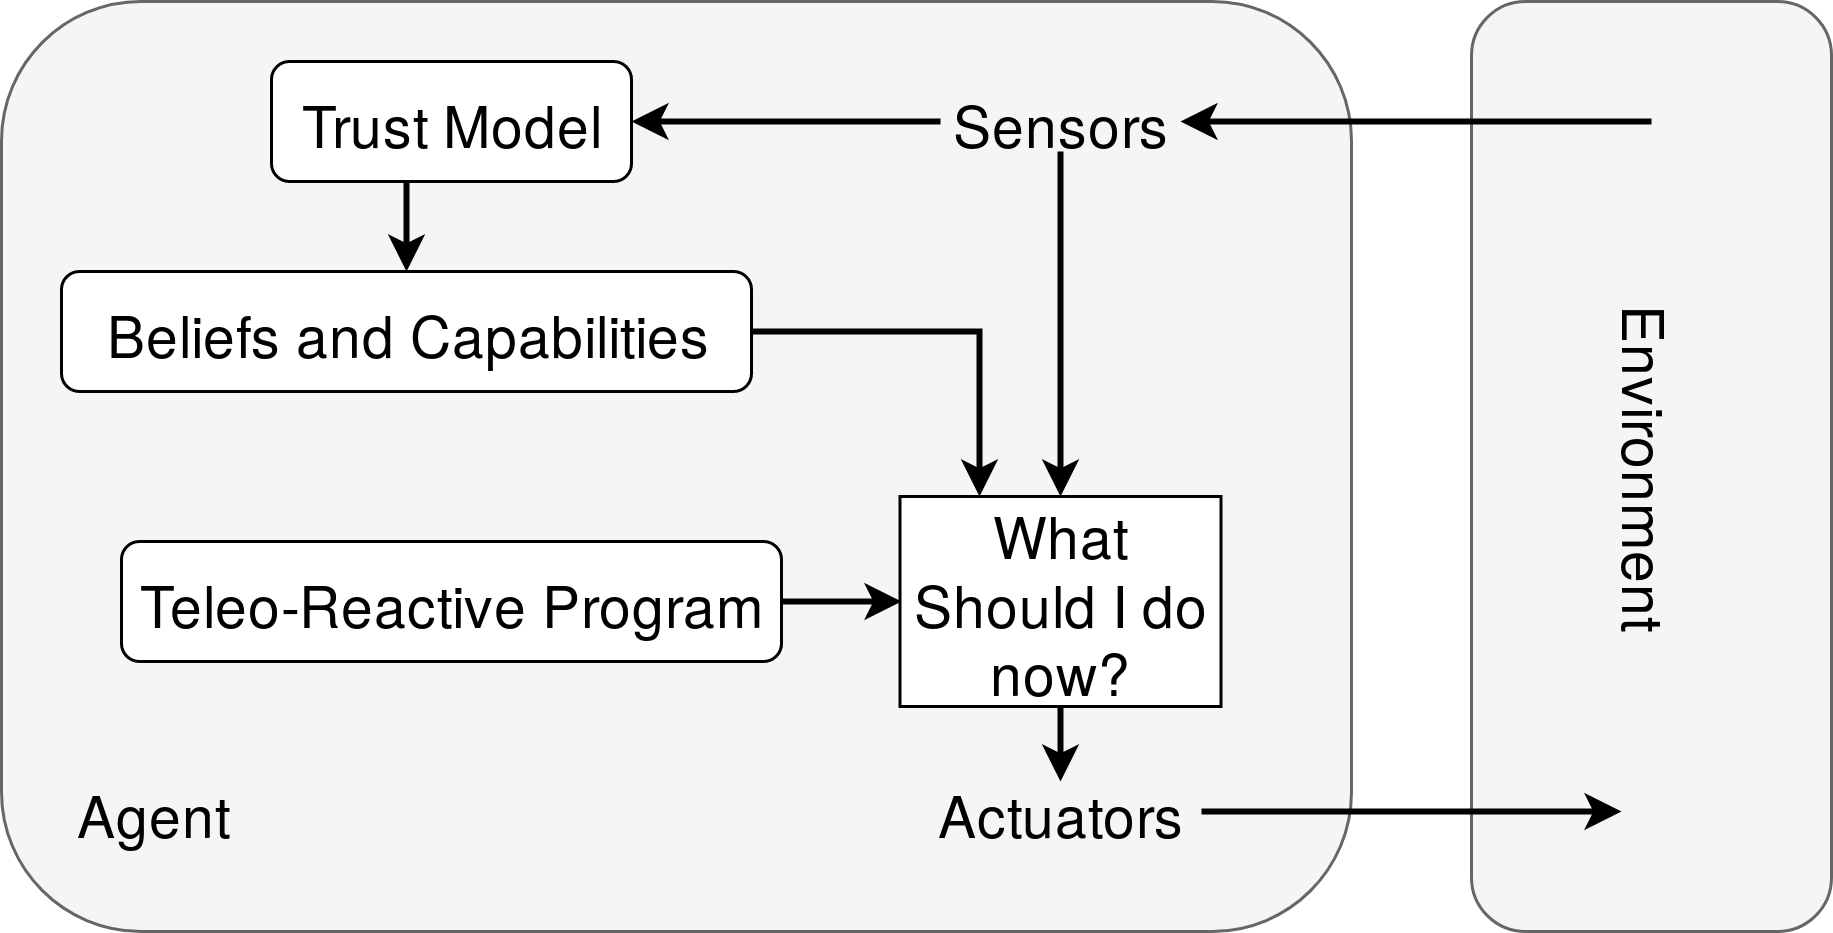
\includegraphics[width=0.5\textwidth]{AgentArchitecture.png}
	\caption{The agent architecture in my system.}
	\label{fig:model_reflex}
	\end{center}
	\vspace{-30pt}
\end{wrapfigure}
The trust model and beliefs system use the multi-valued fluent cached events calculus. The beliefs are a combination of the value and the fluent of multi-valued fluents~\cite{artikis2009specifying}. For example the fluent $standing(agent1, agent2, t)=value$ is the belief of $agent1$ on the standing of $agent2$ at timepoint $t$. In this fluent the value can either be `good' or `bad'. The trust model controls the interpretting of percepts and updating of these fluents.\par
Capabilities are also a part of the beliefs system that are revised during the interpretation of percepts. These capability beliefs constrain an agent as to the actions to which they can commit i.e. an agent can only commit to an action if they believe that they are capable of it. For example, at a time when an agent is a donor in a donor-recipient pair, they will only believe themself capable of a donor action, constraining their action choice.\par 
To make a decision on an action the agent architecture combines the agent's beliefs with a teleo-reactive program that makes up an agent's strategy. A strategy is made up of strategy `components'. Of which one I have already discussed: the trust model. The trust model is combined with a component determining how to act as a donor and another determining how to act when not a donor. The decision is a commitment at that timepoint to carry out that action.

\subsection{Strategies and Trust Models}
\label{subs:stratstrustmodels}
As I have discussed, an agent's strategy is made up of the trust model, the strategy component for when the agent is a donor and the strategy component for the agent when it is not a donor. These strategies have been inspired by past work on indirect reciprocity and expanded upon. For example, I have enhanced agent's interpretation of events in order that they respond differently when they are the recipient of an action from a donor and when they are the recipient of gossip. The action decisions made when agents are donors have generally remained the same as those in past work. However, these action decision systems have been augmented with new strategy components for when an agent is not a donor.\par 
\subsubsection{Defector and Cooperator}
Franklin and Graesser~\cite{franklin1996agent} talked about an agent's primative motivator or drive. Each strategy has a drive or a combination of drives. For example, the `Defector' strategy seeks to protect it's own interests by always defecting, thus not causing it to lose fitness points. The defector strategy has been augmented with three possible strategy components which it can use when it is not a donor: `Lazy', `Spread Negative' and 'Promote Self'.\par
The `Lazy' strategy component always decides on being idle. The `Spread Negative' component randomly spreads negative gossip about other agents in the system. This component simulates what might be known as `fake news': a form of deception and manipulation. The final component is `Promote Self' in which the agent always spreads positive gossip about itself, aiming to increase it's reputation by spreading misinformation and encouraging others to cooperate with the agent using it.\par 
The strategy `Cooperator' aims to maximise social welfare by always cooperating as a donor. I have also augmented this strategy with three components when the agent agent not acting as a donor: `Lazy', `Promote Self' and `Spread Positive'. `Lazy' is the same as for the defector strategy and so to is `Promote Self', although `Promote Self' when used by a `Cooperator' could be seen as coming from a drive to improve cooperation and not to deceive other agents. The third is similar to `Spread Negative' but instead spreads randomly positive gossip in order to improve cooperation between agents in the system. This strategy component could result in accidental manipulation to cooperate with non-reciprocating agents by naive agents.\par 
\subsubsection{Image Scoring Discriminator}
Neither `Defector' nor `Cooperator' have any beliefs about other agents and as such are limited to only trust models that constrain their capabilities. A more insteresting strategy is the `Image Scoring Discriminator'. Built up around Nowak and Sigmund's~\cite{evol_indirect_image} discriminator, strategies using this component keep beliefs about the image score of other agents in the system bounded by $-5$ and $5$. To control these image score beliefs I have created three trust models for these discriminators: `Naive Trusting', `Trusting' and `Distrusting'.\par
The `Distrusting' trust model abjectly ignores any received percepts which it has not observed directly i.e. rejects any gossip. At the other end of the spectrum, `Naive Trusting' accepts any gossip it receives, increasing the image score of the agent the gossip is about by 1 if the gossip is positive, and decreasing by 1 if the gossip is negative. The `Trusting' model is less black and white. This trust model will only change the beliefs regarding the target of the gossip if the gossiper is trusted i.e. has an image score greater than or equal to $k$, where $k$ is an integer variable set at the start.\par
The `Image Scoring Discriminator' strategy component has four corresponding non-donor strategy components. These include `Lazy' and `Promote Self'. Again, it could be said that `Promote Self' is used to improve cooperation towards the agent and not to deceive the recipient.\par
The other two components are `Spread Accurate Positive' and `Spread Accurate Negative'. `Spread Accurate Positive' spreads positive gossip about trustworthy agents to other trustworthy agents. Trustworthy means that their image score is greater than or equal to $k$. The aim of this positive gossip is to improve cooperation between trustworthy agents. `Spread Accurate Negative' spreads negative gossip about agents believed to be untrustorthy - agents with an image score less than $k$ - to trustworthy agents.\par 
It is also possible with agents using image scores to select agents with the `Personal Grievance' option. When this option is selected, agents using the strategy increase or decrease image scores by 2 when respectively receiving a cooperation or defection. These agents use the selected trust model when they are not the recipient of these actions.\par
\subsubsection{Standing Discriminator}
The standing strategy is also included in my system under the name `Standing Discriminator' with the trust models: `Naive Trusting', `Trusting' and `Distrusting'. This strategy has the following strategy components for when the agent is not a donor: `Lazy', `Promote Self', 'Spread Accurate Positive' and `Spread Accurate Negative'. These are the same as for the `Image Scoring Discriminator' strategy components except an agent is said to be trustworthy if their standing is `good'.\par
The original standing strategy specification for when to change an agent's standing between `good' and `bad' is used for directly observed events. The `Personal Grievance' option is not selectable for the standing strategy.

\subsection{The Veritability Discerner}
The image scoring and standing strategies were both built for systems in which gossip was not present and the reliability of the information they received did not require questioning. I have added trust models to compensate for these issues. However, these trust models are built to either accept or to reject the information from the percept and I do not believe that this procedure reflects how reputation information is interpreted in the real world.\par 
Thus, I have developed a new strategy with corresponding trust models and strategy components. I have named this strategy the `Veritability Discerner'. An agent using the strategy holds two beliefs about all other agents. One is the number of percepts the agent has received about the other agent $n$ (when the other agent was a donor or the target of gossip). The second, is an integer value  I have named the `veritability rating' $v$. This rating is initially 0. This rating is similar to an image score but it is not bounded and does not simply increase or decrease by 1, the addition or subtraction to the veritability rating is weighted by the reliability and severity of the percepts.\par 
\subsubsection{Trust Models}
This strategy comes with three trust models: `Strong Reactor', `Balanced Reactor' and `Forgiving Reactor'. All use the same central weighting and reaction system but apply slightly different weights on top of these.\par 
The central weighting and reaction system is as follows. Viewing of a cooperation is the most reliable indication that the donor can be trusted, and so has the highest weight (20) added to the veritability rating of the agent. Conversely viewing a defection against a recipient who is a trusted agent is the most reliable indication that the donor is untrustworthy, and so the highest weight (20) is subtracted from the veritability rating. When either of these interaction events are observed, the count of percepts received about the donor is incremented by 1. Similaryly to the standing strategy, a defection against an untrusted agent has no effect on the veritability rating of the agent but does increment the percept count.\par
Negative gossip about an agent from a trusted source subtracts 10 from the veritability rating of that agent, whilst positive gossip from a trusted source adds 10 to the rating. If gossip is from an untrusted source, then only 1 is respectively added or subtracted from the rating.\par 
The `Strong Reactor' trust model multiplies weights for negative percepts by 2. This multiplication makes the weight for defection against a trusted recipient 40. The multiplication also makes negative gossip from a trusted source subtract 20 from the veritability rating of the target of the gossip. The last effect the multiplication has is to cause a subtraction of 2 from the veritability rating of the target of gossip in response to negative gossip from an untrusted source.\par 
The `Balanced Reactor' does not apply a weight to either positive or negative percepts. Finally the `Forgiving Reactor' multiplies positive weights by 2, making the weight of viewing a cooperation 40, positive gossip from a trusted source 20 and positive gossip from an untrusted source 2.
\subsubsection{Trustworthiness}
A third belief can be derived from the veritability rating and count of percepts received: trustworthiness. An agent using the strategy has a value $k$ similar to an `Image Scoring Discriminator' agent, though the possible values for this are -10, -5, 0, 5 and 10. The trustworthiness belief is derived as follows. Divide the veritability rating by the count of the percepts received $v/n=t$ - if $n$ is 0 $t$ defaults to 0. If $t\ge k$, then the agent is trustworthy, otherwise they are untrustworthy.
\begin{framed}
		\begin{flushleft}
			\vspace{-20pt}
			$holds\_at(veritability\_rating(Perceiver, Subject)=V, Timepoint)\ \wedge$\\
			$holds\_at(percept\_count(Perceiver, Subject)=N, Timepoint)\ \wedge$\\
			$get\_K(Perceiver, K)\ \wedge V/N \ge K \rightarrow $
		\end{flushleft}
		\vspace{-30pt}
		\begin{flushright}
			$trustworthy(Perceiver, Subject, Timepoint)$
		\end{flushright}
		\vspace{-10pt}
\end{framed}
The derivation of this belief has the same effect as taking the mean of a list of weighted actions. This mean takes into account all the actions committed to by an agent but smooths out noise from possibly untrustworthy or distorted sources.\par
The trustworthiness belief about an agent is used when intepretting gossip and when deciding whether another agent's defection was justified or not. This belief is also used for when the agent is a donor. If the recipient is considered trustworthy then the agent will cooperate, if they are not, the agent will defect.
\begin{framed}
		\begin{flushleft}
		\vspace{-20pt}
			$get\_strategy(Actor, ``Veritability Discerner")\ \wedge$\\
			$interaction\_pair(Actor, Recipient, Timepoint)\ \wedge$\\
			$trustworthy(Actor, Recipient, Timepoint)\ \rightarrow$\\
		\end{flushleft}
		\vspace{-30pt}
		\begin{flushright}
			$action\_commitment(cooperate, Actor, Recipient, Timepoint)$
		\end{flushright}
		\vspace{-10pt}
\end{framed}
\subsubsection{Strategy Components}
Finally we need strategy components for when an agent using the strategy is not a donor. These are similar to the discriminator strategies and include: `Lazy', `Promote Self', `Spread Positive Trusted' and `Spread Negative Untrusted'. `Lazy' and `Promote Self' do the same as with all other strategies. `Spread Positive Trusted' spreads positive gossip to trusted agents about trusted agents. `Spread Negative Untrusted' spreads negative gossip to trusted agents about untrusted agents.\par
`Spread Positive Trusted' formalisation:
\begin{framed}
		\begin{flushleft}
		\vspace{-20pt}
			$get\_strategy\_component(Actor, ``Spread\ Positive\ Trusted")\ \wedge$\\
			$not\ interaction\_pair(Actor, _, Timepoint)\ \wedge$\\
			$findall(Trusted, trustworthy(Actor, Trusted, Timepoint), TrustedAgents)\ \wedge$\\
			$len(TrustedAgents, Len)\ \wedge Len >= 2\ \wedge$\\
			$get\_2\_random(TrustedAgents, TrustedAgent, Recipient)\rightarrow$\\
		\end{flushleft}
		\vspace{-30pt}
		\begin{flushright}
			$action\_commitment(gossip(\{recipient: Recipient, about: TrustedAgent, gossiper: Actor, timepoint: Timepoint, gossip: positive\}), Actor, Recipient, Timepoint)$
		\end{flushright}
		\vspace{-10pt}
		\begin{flushleft}
			$get\_strategy\_component(Actor, ``Spread\ Positive\ Trusted")\ \rightarrow$\\
		\end{flushleft}
		\vspace{-30pt}
		\begin{flushright}
			$action\_commitment(idle, Actor, Recipient, Timepoint)$
		\end{flushright}
\end{framed}
`Spread Negative Untrusted' formalisation:
\begin{framed}
		\begin{flushleft}
		\vspace{-20pt}
			$get\_strategy\_component(Actor, ``Spread\  Negative\ Untrusted")\ \wedge$\\
			$not\ interaction\_pair(Actor, _, Timepoint)\ \wedge$\\
			$findall(Trusted, trustworthy(Actor, Trusted, Timepoint), TrustedAgents)\ \wedge$\\
			$len(TrustedAgents, Len)\ \wedge Len >= 2\ \wedge$\\
			$get\_random(TrustedAgents, Recipient)\rightarrow$\\
		\end{flushleft}
		\vspace{-30pt}
		\begin{flushright}
			$action\_commitment(gossip(\{recipient: Recipient, about: TrustedAgent, gossiper: Actor, timepoint: Timepoint, gossip: positive\}), Actor, Recipient, Timepoint)$
		\end{flushright}
		\begin{flushleft}
			$get\_strategy\_component(Actor, ``Spread\ Negative\ Untrusted")\ \rightarrow$\\
		\end{flushleft}
		\vspace{-30pt}
		\begin{flushright}
			$action\_commitment(idle, Actor, Recipient, Timepoint)$
		\end{flushright}
\end{framed}
\subsubsection{Summary}
I have presented a new strategy for use in indirect and direct reciprocity models. The aim of this strategy is to be less susceptible to deception and manipulation by weighting the increase and decrease of the ratings by the severity and reliability of the percepts and also by using the smoothing properties of the arithmetic mean. 

\subsection{Summary}
In summary, I have presented a MAS that uses a variant of a genetic algorithm to reproduce agents between instances of the environment. I have described the components of the environment and game, the percepts that can be received by agents, the actions available to agents and how these are constrained and the simple agent gossip language. I have also discussed the architecture that I am planning to use in the system and the strategies and trust models available to associate with the agents, including a new strategy that aims to be more suitable with a system in which deception and manipulation are possible.

\section{Implementation}
\subsection{Introduction}
In this section I will discuss the details of the implementation of the theoretical framework outlined above as well as the architecture of the system that is hosting it. I will also be discussing the software engineering techniques, tools and processes I have employed in the development of my system.

\subsection{Development}
\subsubsection{Architecture}
\begin{wrapfigure}{l}{0.5\textwidth}
\vspace{-30pt}
\begin{framed}
	\begin{center}
	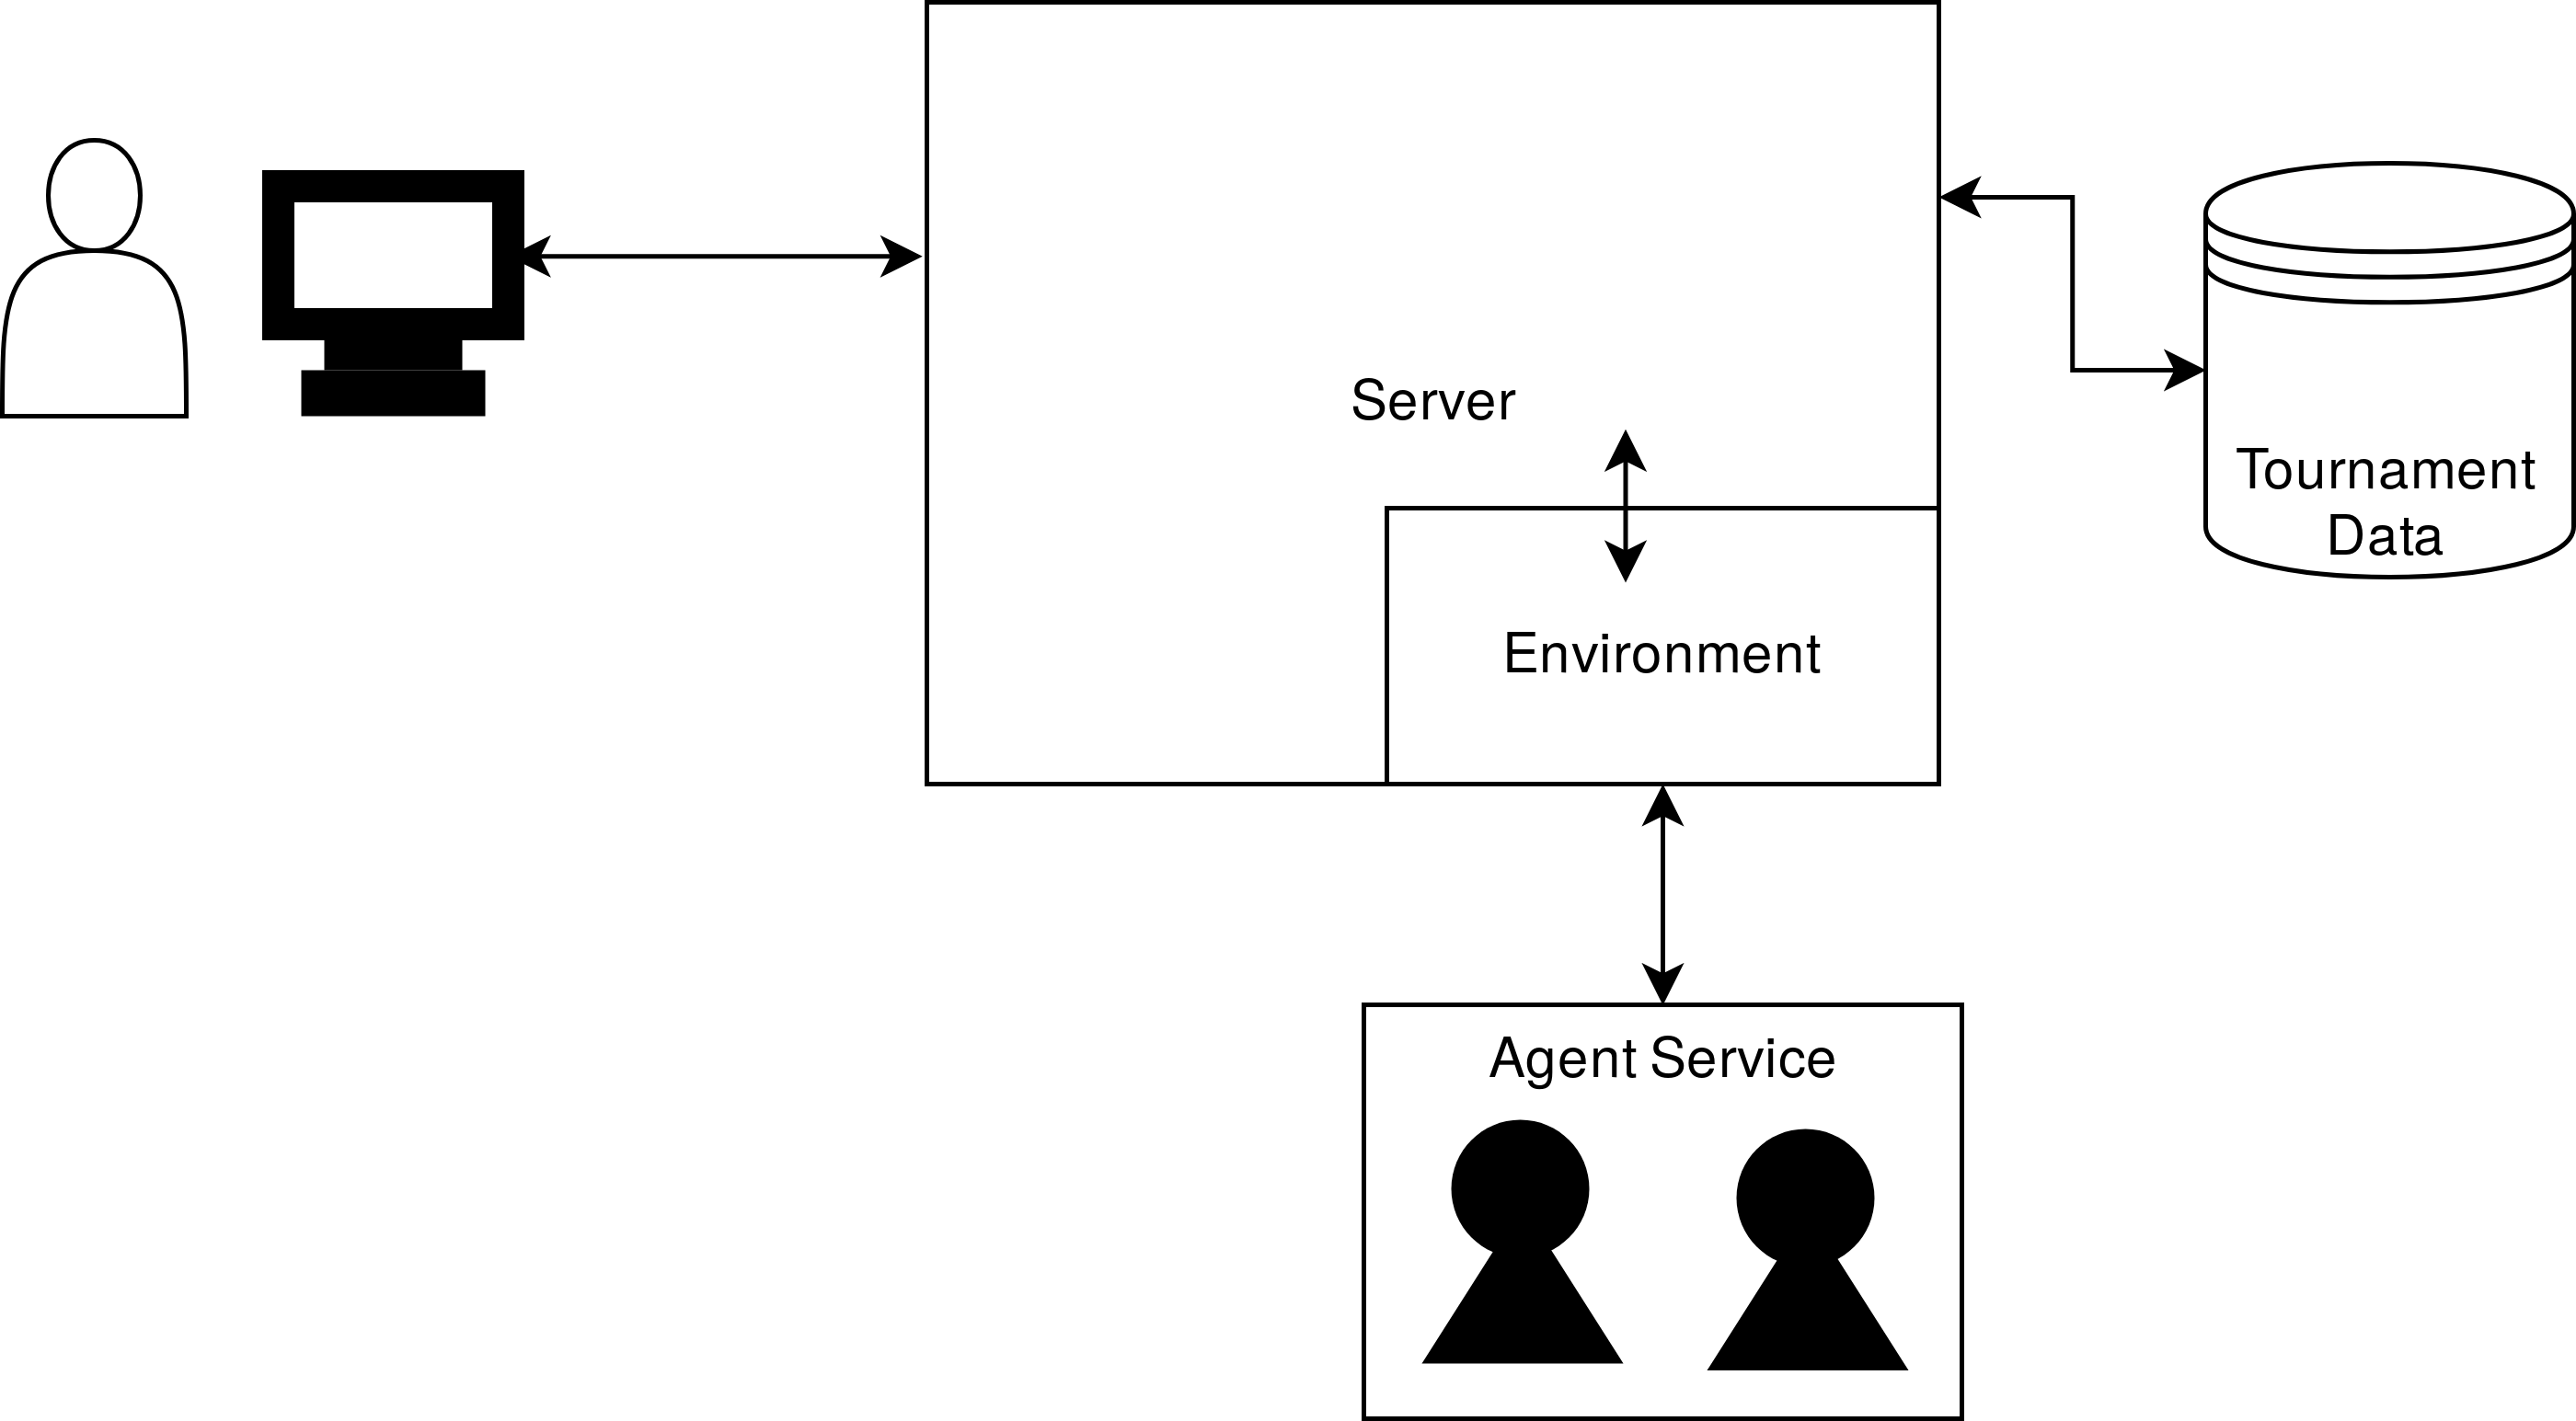
\includegraphics[width=\textwidth]{PresSystem.png}
	\caption{System architecture}
	\label{fig:architecture}
	\end{center}
\end{framed}
\vspace{-30pt}
\end{wrapfigure}
One of the objectives of my project is to create a system that is distributable, in order for it to be an experimentation and learning tool for those interested in studying multi-agent interactions. This distributability is reflected in the architecture I have used to develop my system. A web application acts as the `shop front' of the system and allows anyone with internet access to create, run and view analysis of the available games.\par 
I named the web application `The Nature Engine' and it is of typical web architecture: the client-server model. Built into this web application is an implementation of my theoretical framework which runs the environment and the agent's bodies. Notably this part of the system doesn't include agent decision making components. These components are hosted in a separate web service, that has been named the Agent Mind as a Service (AMAAS). This web service exposes an API for the web application to interact with.\par 
The final component of the system is a database for the long term storage of data about users of the site (to enable users to record and label experiments) and game data. This is a relational database that due to the use of and ORM (SQLAlchemy) I have been able to create as both SQLite for development and MySql for deployment. An illustration of this is in figure~\ref{fig:architecture}. The system is deployed on an ubuntu server and the database is situated on another machine.


\subsubsection{Proof of Concepts and Learning}
At the very beginning of this project I had a good amount of software development experience, some experience with database development and logic programming, and less experience with web development. Before undertaking the development I decided I needed to learn more about some of these areas (especially web development).\par 
I had decided that I wanted to extend my experience with Python due to it's nice language features, good library support and it's lack of use in the development of MASs (in comparison to Java and Prolog). As such I decided to use the Flask web development micro-framework and partake in Miguel Grinberg's course "The Flask Mega-Tutorial"~\cite{flask_tut}. Flask is a micro-framework as it only includes a minimal amount of functionality in comparison to frameworks such as Django. Nevertheless Flask is extensible and there are a lot of libraries a programmer can use to bring in required functionality.\par 
Using inspiration and the techniques learnt in this course I developed an early prototype of The Nature Engine. This prototype provided a number of web pages and navigation between them including a home page, pages to set up and run two player iterated prisoner's dilemma games and pages to set up and run tournaments of the iterated prisoner's dilemma and the respective analysis of both game types. Both of these games are run using the Axelrod-Python library~\cite{axelrodproject}. This early prototype also included a database set up, a redis queue to run the tournaments and a front-end that used bootstrap for styling and React.js for a dynamic form to set up tournaments.\par
\begin{figure}
\begin{framed}
\begin{subfigure}{.55\textwidth}
	\begin{center}
	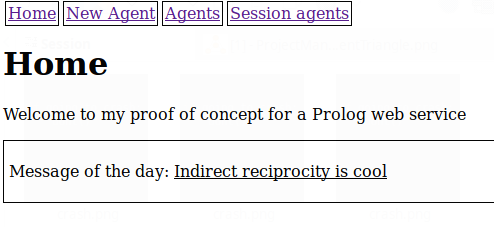
\includegraphics[width=\linewidth]{PrologServiceProof1.png}
	\end{center}
\end{subfigure}
\begin{subfigure}{.45\textwidth}
	\begin{center}
	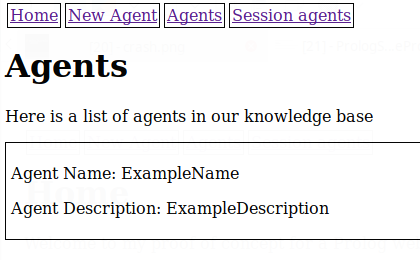
\includegraphics[width=\linewidth]{PrologServiceProof2.png}
	\end{center}
\end{subfigure}
\end{framed}
\caption{Two screenshots of two pages of the Prolog web service proof of concept}
\label{fig:prologproof}
\end{figure}
Prolog is a logic-language traditionally used for the development of symbolic AI systems. The language allows a programmer to elegantly lay out how an agent makes decisions and interprets percepts. There are limited libraries for interfacing between Prolog and Python, and creating a method for interfacing between them reliably would have taken a while. It was easier to create a web service to host agent minds and became a good opportunity to hone my skills in web development.\par 
To develop these skills I used Anne Ogborn's `Creating Web Applications in SWI-Prolog' tutorial~\cite{swi_web_tut} and the swi-prolog documentation. Using this tutorial I created a basic web application that imitates managing the creation of strategies and agents within the system. This was far simpler than The Nature Engine prototype (figure~\ref{fig:prologproof}) as it did not build up to a final application (the development of AMAAS was separate to this proof of concept).

\subsubsection{The Nature Engine}
I built on top of the early prototype of The Nature Engine to develop the final web application. This included improving the front end content, adding a section to run the theoretical framework I have devised and adding a couple of extra features.\par 
To improve the front end content I worked on improving the form that allows users to dynamically select and remove agents from a tournament. This also translated into the form that allows users to do the same for my game. Other improvements were the use of a bootstrap carousel for the homepage to prevent text overload on the screen, better text descriptions on the website and improved game and tournament analysis.\par 
\begin{wrapfigure}{l}{0.7\textwidth}
\vspace{-30pt}
\begin{framed}
	\begin{center}
	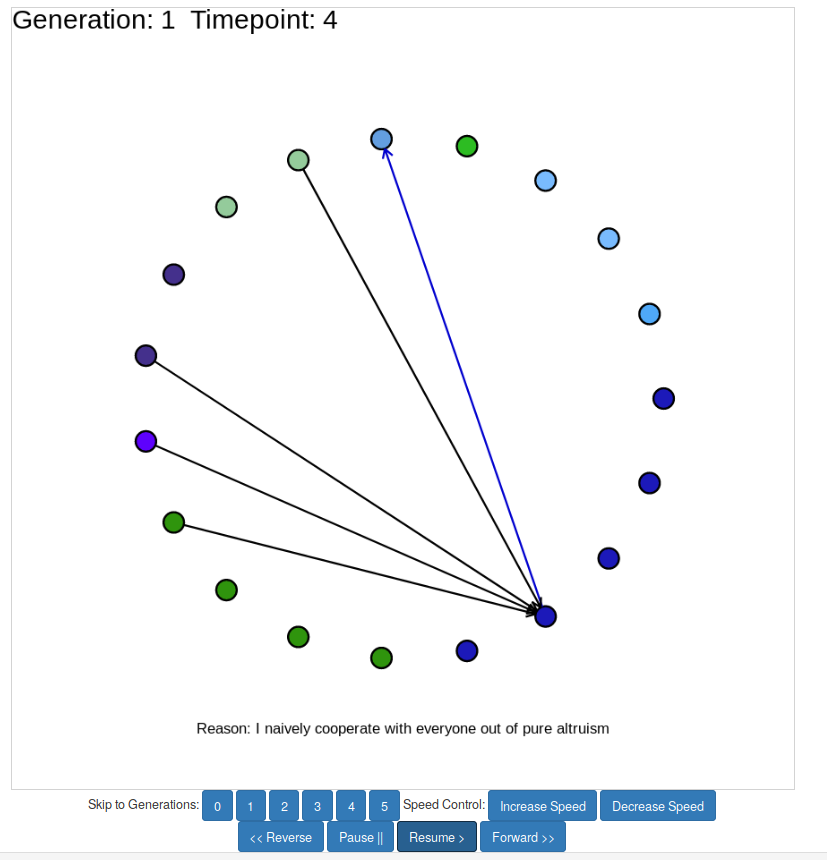
\includegraphics[width=\textwidth]{Animation.png}
	\caption{The animation of a game.}
	\label{fig:animation}
	\end{center}
\end{framed}
\vspace{-30pt}
\end{wrapfigure}
The main bulk of the development was implementing the theoretical framework. However, to run this game in the web application required a front-end, processing of user requests and storing of data in the database. This development is a vertical slice of the web application. The process is as follows. A user sets up a game on the set up page using a React.js form (decisions are informed by strategy information in an information box), this form is submitted which sends a post request with the relevant information to the server.\par 
\begin{wrapfigure}{l}{\textwidth}
\vspace{-30pt}
\begin{framed}
	\begin{center}
	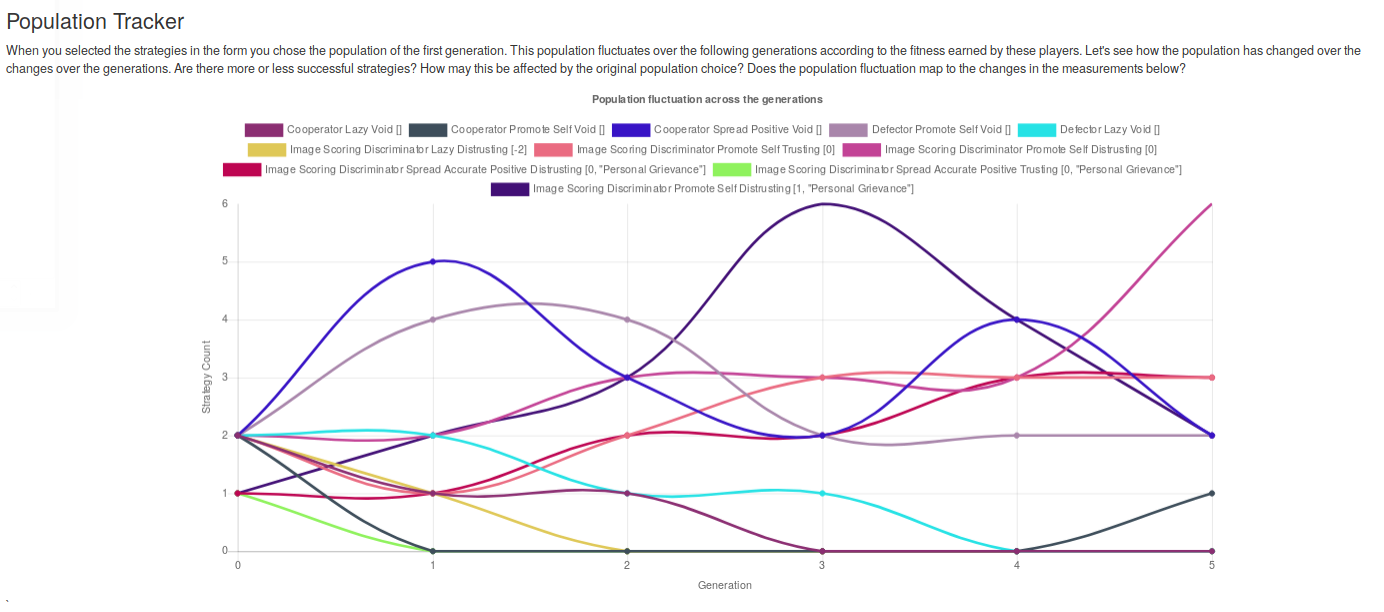
\includegraphics[width=\textwidth]{PopulationTracker.png}
	\caption{Tracking the population of strategies through each generation.}
	\label{fig:population_tracker}
	\end{center}
\end{framed}
\vspace{-30pt}
\end{wrapfigure}
The server then puts a method to create and run the game in a redis queue and then store the resulting data in the database. The user is redirected to a waiting page, which either notifies them of a timeout on their game or sends them through to the analysis page. The analysis page includes a run down of the statistics in terms of cooperation, gossip and the success of each strategy and agent. A visualisation of the game that has been run is also included in an animation on the analysis page.\par 
\begin{wrapfigure}{l}{\textwidth}
\vspace{-30pt}
\begin{framed}
	\begin{center}
	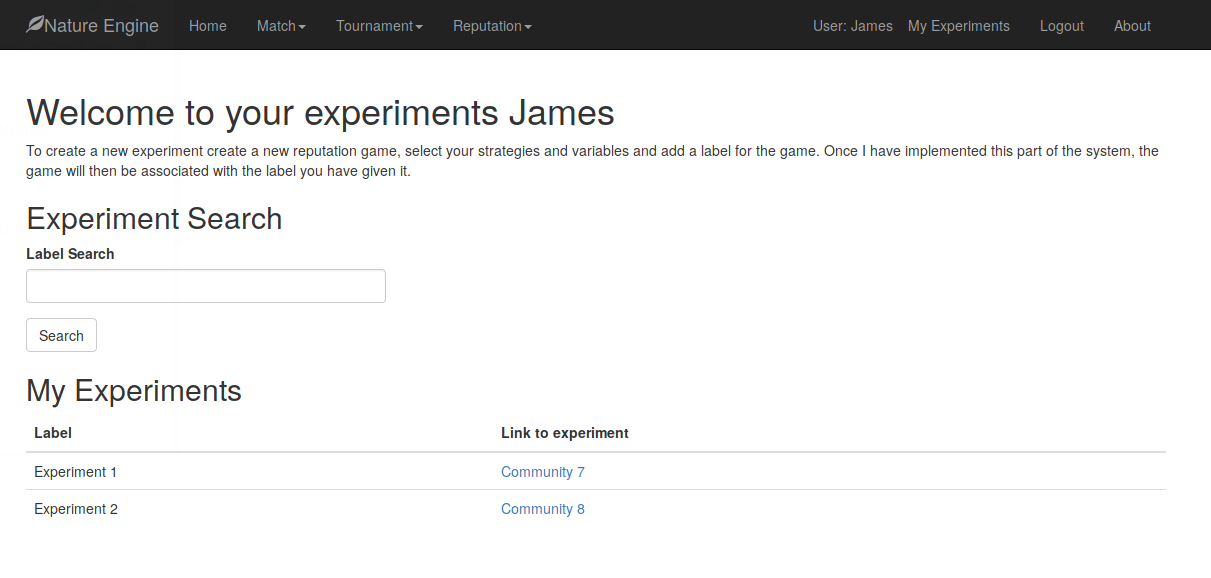
\includegraphics[width=\textwidth]{UserExperiments.png}
	\caption{The user experiment tracker}
	\label{fig:user_experiments}
	\end{center}
\end{framed}
\vspace{-30pt}
\end{wrapfigure}
In addition to this I have created a feature that allows users to create accounts, login and associates games of my theoretical framework to their account. These games can be given a label so they can keep track of the experiments the have run (illustrated in figure~\ref{fig:user_experiments}). User data is recorded in the database and passwords are hashed to keep them secret.\par
The web application, database and AMAAS system has been deployed to an Ubuntu Server and has a domain name (natureengine.tech) that is accessible to all across the internet.

\subsection{Framework}
\subsubsection{Introduction}
In this section I will lay out the implementation of the environment, agents and strategies I have described in the theoretical framework (section~\ref{sec:theo}). 
\subsubsection{Environment and Agent's Bodies}
The environment and agent's bodies from the theoretical framework described in section~\ref{sec:theo} has been implemented within the nature engine web application in it's own package. As such the environment and agent's bodies components have been written in Python.\par 
This has taken an object oriented approach. A Community object is the overarching object that simulates the specified number of generations and handles the reproduction of strategies between generations assigning the strategies that should be associated with players in a Generation. A Generation object creates a set of players from these passed strategies.\par 
The Generation is then simulated. Simulation of a generation involves running the synchronised cycle steps from the start timepoint of that generation to the end timepoint. In each perceive step a donor-recipient pair is selected at random by a method of the Generation object and the relevant agents are notified.\par 
In the previous timepoint a set of percepts is generated - from the actions of that timepoint - for the current timepoint and are set into the perception bank ready to be transmitted at the current timepoint. These are sent in the perceive step. Agents are then asked to decide on an action at the current timepoint. Once these actions have been returned to the Generation they are executed, affecting players fitness and generating more percepts.\par 
A Player is also an object in the system, and is associated with a strategy that describes how it should act at each timepoint. The Player object handles the sending of percepts and getting of actions from their decision making component in the AMAAS system. The Player object also encapsulates the player's state including the fitness of that player.\par 
The 3 classes that implement the Action abstract class represent the three possible types of action that are available and the relevant data associated with an instance of an action.

\subsubsection{Agent Mind as a Service (AMAAS)}

The AMAAS system was developed in Prolog. This system handles the management of communities, generations and agents by assigning them with an ID generated using a similar system to the Prolog gensym library. These are assigned to the predicates $community(CommunityID)$, $generation(Community, GenerationID)$ where $Community$ unifies with a community and $agent(Strategy, Community, Generation, AgentID)$ where $Strategy$ unifies with a strategy in the system and Generation with a generation.\par
the community/1, generation/2 and agent/3 predicates are dynamic and can be asserted and retracted. The possible strategies that unify with $Strategy$ are not dynamic and are defined with a strategy predicate (strategy/5). The first 4 arguments are strings and are in the correct order: the strategy to use when a donor, the strategy to use when not a donor, the trust model, the description of the strategy. The final argument is a list of any type that contains options to augment the strategy that are not a necessity to define for every strategy.\par 
Some of the available strategies (any associated with the donor strategies ``Standing Discriminator'', ``Image Scoring Discriminator'' and ``Veritability Discerner'') hold beliefs about other agents and the environment. These beliefs are stored with fluents in the MVFCEC. The value of these fluents are revised by the definition for initiates\_at/4 and terminates\_at/4 of that agents strategy and trust model and the events and conditions that cause these predicates to fire.\par
These predicates are caused to fire by the receiving of percepts to the agents service that then asserts a new event observation (the observed\_at/2 predicate) and calling an update on the MVFCEC using the update\_at/2 predicate. The process of firing these is controlled for all possible percepts by the add\_new\_action\_gossip\_percept/2, add\_new\_action\_interaction\_percept/2 and add\_new\_interaction\_percept/2 predicates.\par
The beliefs formed by the firing of these predicates and the initiating and terminating of fluents is then used by the teleo-reactive program created for each strategy to decide on actions at certain points in time. An agent decides on an action by the firing of the agent\_action/6 predicate. A set of agent\_action/6 definitions is given for each donor and non-donor strategy. The first four arguments are input arguments being the timepoint to decide at, the id of the community and the generation the agent belongs to and finally the id of the agent.\par 
The second to last argument stores true if a decision has been successfully made or provides an error message if it has not been. The last argument unifies with an action (the dictionary representation of that action). The program is teleo-reactive as the system is designed so only one of the bodies of the set of agent\_action/6 definitions satisfies the conditions required, and this forces unification with one action.\par 
The higher level predicate get\_action/6 checks if an agent has already committed to an action at a specific timepoint. This predicate also ensures that an agent only commits to actions that it believes it is capable of using capable/5 predicate, which is only satisfied if the agent is committing to a donor action as a donor or a gossip or idle action if it is not a donor.

\subsubsection{Simple Agent Gossip Language}
The specification of SAGL (subsection~\ref{subs:sagl}) is remarkably similar to data structures used in Python (Dicts), the JSON structure and dictionaries in Prolog. As such, it made sense to implement SAGL by storing it as Python Dicts in the environment and agent's bodies, transferring it with JSON (as is used for the API in general) and then storing it as dictionaries in Prolog. 

\subsection{Software Engineering}
\subsubsection{Introduction}
In this section I will discuss and reflect on engineering tools, techniques, methodologies and approaches that I have used, and some that I possibly should have used.

\subsubsection{Process}
The development process I decided on when starting the project was a scrum like structure, with a task backlog that was subject to change and fortnightly sprints. Although I have mostly stuck to these sprints, the backlog was in constant flux, far more than was expected. This is likely due to me still learning lots about the topic during the project. This was not due to a lack of research, but a focus on game-theory over multi-agent system design.\par 
I feel that I could have managed this better with a more structured approach to design of the system, and by opening up my focus to all areas of the topic. However, I believe this structure allowed me to be open to new ideas and aspects to add to the project. I was then able to incorporate aspects of multi-agent systems and game-theory fields I may have not been able to with a more structured approach.\par 
As it was, the design phase of the process was greatly interleaved with both learning the concepts for designing the system and the implementation of it. The implementation of the system then followed a Test-Driven Development (TDD) approach, developing tests and then creating code to work for those tests, and afterwards refactoring. This followed with a deeper more fully encompassing testing using a bottom-up integration testing strategy.\par 
This highly interleaved process worked quite well for my project as it allowed me to design, develop and test features in the system separately all in the same slice of tasks. This process also allowed me to discover new features, ideas and strategies to incorporate in the system and then extend the project by adding a new slice of tasks to the task backlog which I could then choose when to implement based on urgency and importance.\par 
I followed a bottom-up strategy when developing the components of the system. The multi-agent system is dependent on the agents service being fully functional and safe to use. As such I focused on developing and testing the AMAAS system and a base set of strategies for this first.\par 
From this I then developed and tested a base set of components for the environment of the MAS. Once I had a safe and working base system I incorporated the MAS into the web application. From there I worked on adding new strategies and testing them in the AMAAS system, and then onto adding features to the multi-agent system such as the selection of onlookers and the reproduction mechanism.\par 
This incremental development using slices of tasks for each feature allowed me to be secure that the developed parts of the system were safe for use by other parts of the system.

\subsubsection{Design}
Most of the early design of my system went into learning how the operation of a MAS works, and drawing from multiple sources how to implement it myself. Further to this, I researched agent architectures and fused together multiple styles of design into my own. Both the design of the environment and agents can be viewed in my theoretical framework section (section~\ref{sec:theo}).\par 
I designed the API for the AMAAS system using a RAML specification and then added to this as I went along. This drove the design and implementation of the AMAAS system, by designing what I needed from the service I derived what I needed to implement for the functionality. I also created a theoretical design for the strategies in the system using logical predicates, to translate into Prolog.\par 
The environment and agent's bodies for the multi-agent system were developed using the OOP features of Python. To approach this I used object-oriented design UML design tools (UMLet), and added to this as I enhanced the features of the system. This included a UML class diagram for designing the environment and agent body class structure (figure~\ref{fig:class}) and a sequence diagram to portray the message passing sequence (figure~\ref{fig:sequence}).\par 
In the design of the environment classes I included an observer design pattern to observer player states and collect data on the player and their actions throughout the course of the game. I then created a facade for this so a simple Results class is returned after an object of the ReputationGame type has been run. The ReputationGame class is also a facade on the simulation of the communities and generations, making the system easy to set up a game with (preventing the need to know the underlying implementation).\par 
This project is not focused on interface design and I have not researched or learnt any strategies for user experience design. However, with the knowledge I have of bootstrap components, css and some web development I developed templates for the client side as an informal method of design. I then refined these templates to improve the user experience simply by using the system and noticing any annoyances or issues I had with it.
\begin{figure}
	\begin{flushleft}
	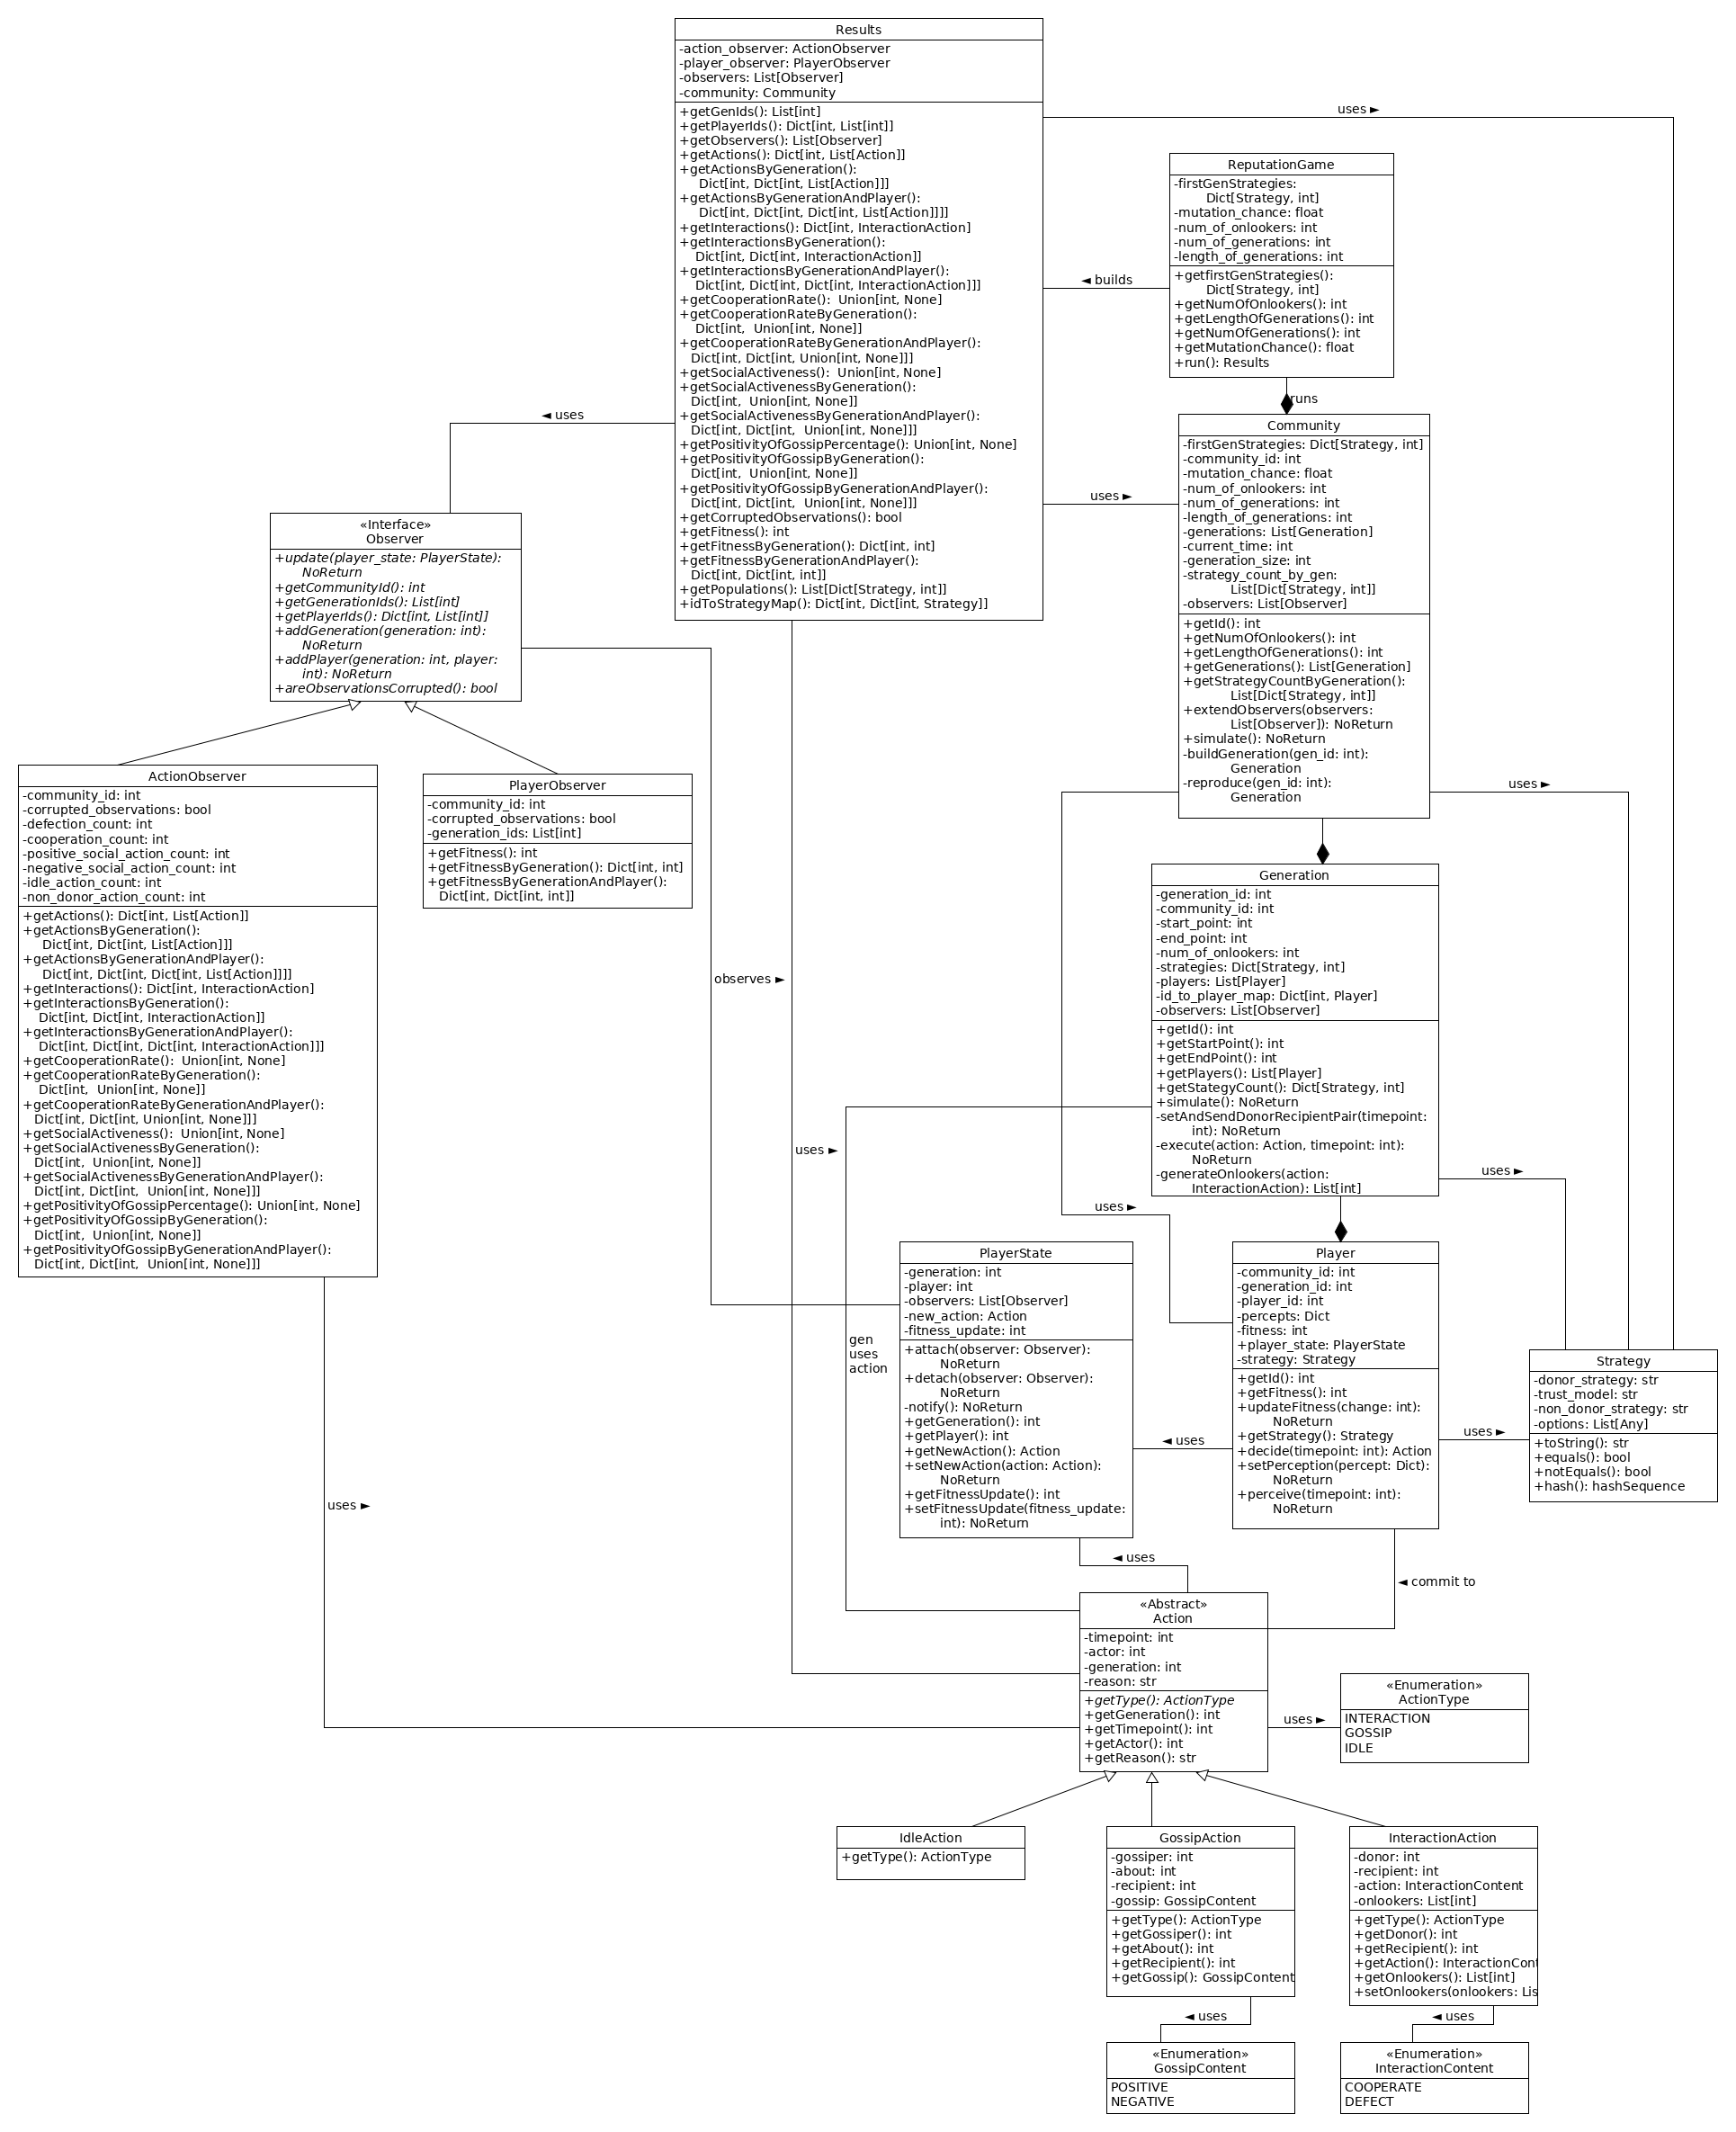
\includegraphics[width=\textwidth]{EnvClass.png}
	\caption{The class diagram for my environment and agent bodies Python program, also can be found in the ProjectReports/NewFinalReport directory as EnvClass.png}
	\label{fig:class}
	\end{flushleft}
\end{figure}
\begin{figure}
	\begin{center}
	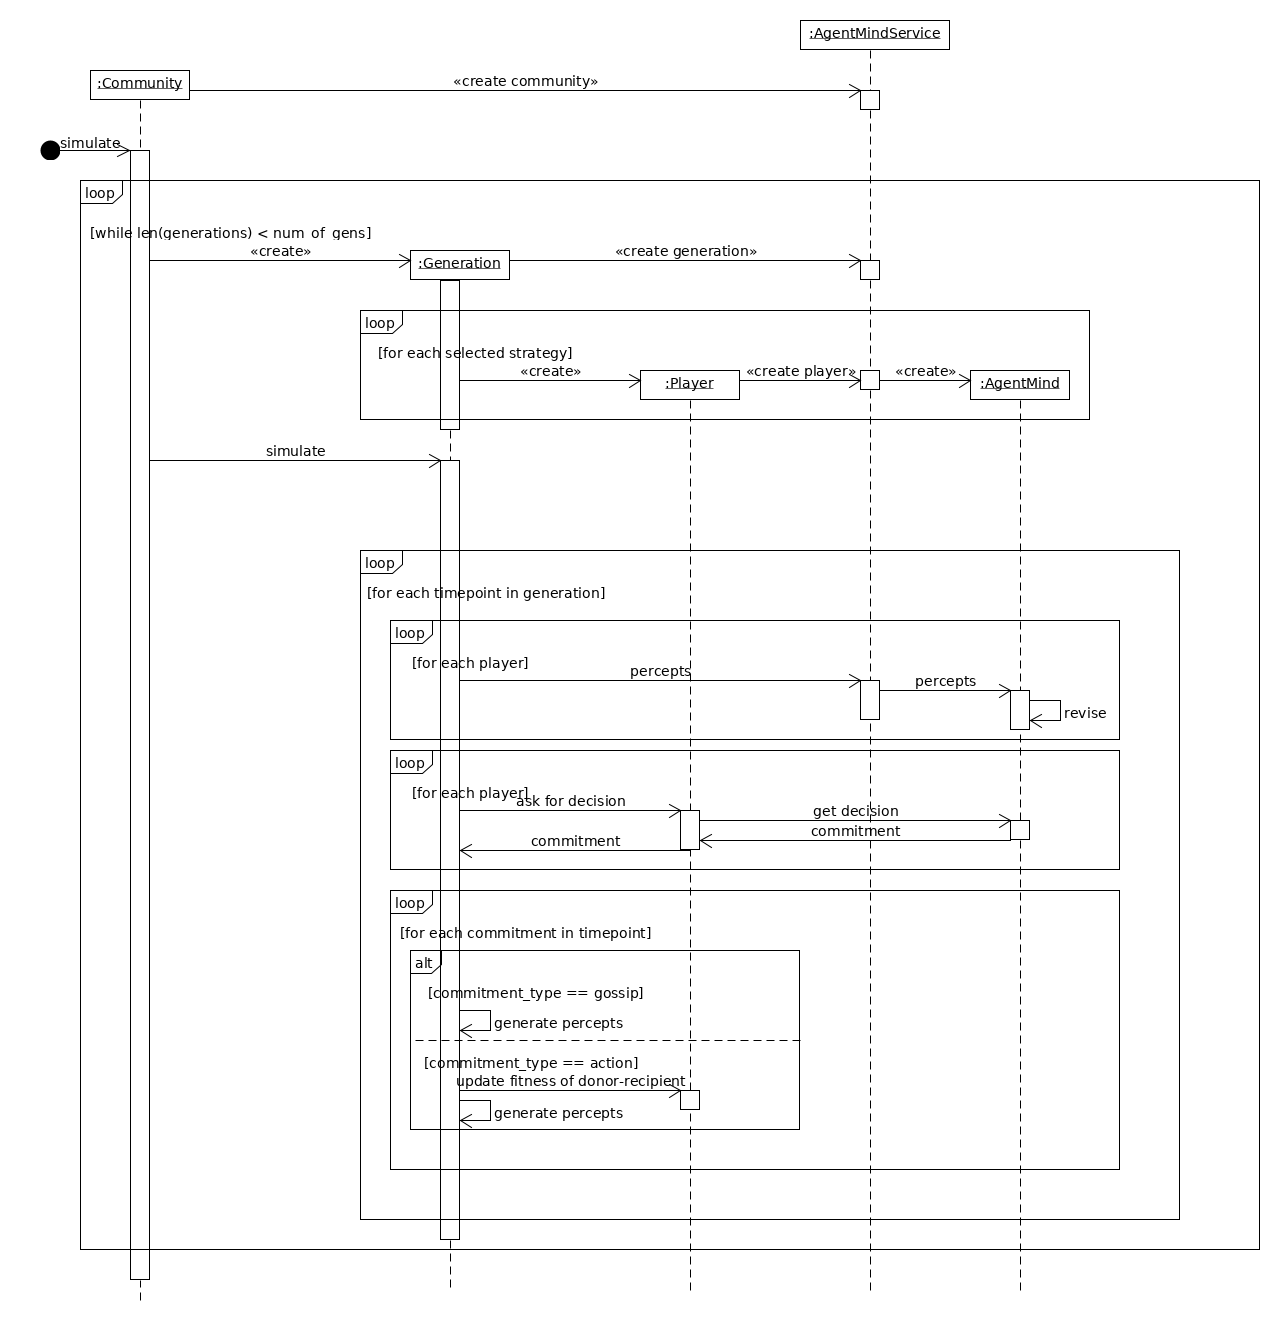
\includegraphics[width=\textwidth]{EnvSequence.png}
	\caption{The sequence diagram for my environment and agent bodies Python program, also can be found in the ProjectReports/NewFinalReport directory as EnvSequence.png}
	\label{fig:sequence}
	\end{center}
\end{figure}

\subsubsection{Development}
As I have mentioned the development phase has been strongly interleaved with testing and design to ensure the safety and correct running of the program. This included a TDD approach to development. I used a number of tools to assist me in this development.\par 
The Python code that I have written follows the PEP 8 Style Guide. I used the Flask web application microframework to assist me in developing the web application and for the creation of the database I used the SQLAlchemy ORM. With SQLAlchemy way I was able to generate for both SQLite (for development) and MySQL (for deployment) databases from Python code. The use of SLQALchemy also assists in the prevention of SQL injection attacks that websites so often fall prey to.\par 
I also used git as a version control system tool, with a master branch and various feature branches which I would develop features on and then once stable merge back into the master. The repository is hosted on GitHub. I mostly used the git command line tool for Linux, however I occasionally used the git support in the PyCharm integrated project support environment.\par 
Pycharm provides more than just version control system tools. There is also a linter and support for the Python language, as well as Jinja2, HTML, CSS and Javascript which I used for front-end development. I have often used the visual debugger, Python environment setup support, Flask support and unittest library support.\par 
There is far less tooling available for Prolog development. I ended up using a mix of Visual Studio Code as it has a linter that helped me catch errors earlier (though I would not recommend this, as it often crashes) and Sublime Text (limited to syntax highlighting).\par 
Again with the development of the AMAAS system I followed a TDD approach, writing unit tests using the PLUnit library. I documented this code using the PLDoc library. There is a good HTTP library for Prolog, that allowed me to easily create a web service with handlers for certain routes that easily link up to functionality in the AMAAS system.


\subsubsection{Testing}
The testing of my system can be broken down into four parts: AMAAS bottom up integration testing, environment bottom up integration testing, application programming interface (API) testing and some extra early unit testing on other parts of the web application. The bulk of this testing comes from the first two, which were interleaved with the development of the system. The early unit testing was also interleaved with development. However API testing was carried out after development.\par 
As the AMAAS system has been developed in Prolog, the unit testing has been done with the PLUnit library. This focused on testing the functionality provided by the predicates I have created in the system. In depth testing has been undertaken for every strategy, in many different possible situations and timelines. I have also tested all predicates for managing agents, generations and strategies in the system as well as the predicates used for receiving percepts and getting actions.\par 
Further to this the AMAAS system has been web API tested. The functionality that the API uses in the system has been thoroughly tested in the bottom up integration testing. As such, API testing focused on ensuring the API met the specification laid out in the documentation. I carried out this testing using the python unittest testing framework and the requests library. I had previously planned on using an API testing tool such as postman, but had found no free and easy way to put my tests into code to put on my github repository.\par 
I also used this testing framework for bottom up integration testing of the environment for my game. This testing also requires the AMAAS system to be running and working correctly so acts as integration testing between the two systems. The testing was interleaved with development in a way that as I created each unit (class) or added functionality to that unit I added testing for the functionality added. I used the same framework for some earlier testing in the web app. This was mostly testing for converting produced game data for the database.\par 
I would also like to have tested the web application including functionality, usability and compatibility testing~\cite{guru99_testing, software_testing_help}. I have developed the user interface to what I believe to be a good standard, but I'm sure it can be improved and it would be good to get feedback to understand where I can improve this. I also have developed the web application so it is responsive using the Bootstrap 3 library, and have used the website on Firefox on Android and Linux, and Chrome on Windows. It would be good to find out the compatibility with Safari and have more eyes to spot bugs in the functionality.

\subsubsection{Documentation}
In the API testing phase I tested the API against the claimed functionality in the API documentation. I created the specification for this documentation in the RESTful API Modelling Language (RAML) which is based on YAML specifically for the creation of RESTful API specifications. There is a good set of tools surrounding RAML, including a linter in the Atom text editor and the raml2html tool that creates a nicely laid out web page for a user readable documentation. I used this tool to convert my .raml file into a .html for readability. This documentation can be found by opening the main.html document in the AgentsService/api\_docs directory in a web browser.\par 
I have also created documentation for the web application code. This is done in the form of writing python docstrings in the reStructuredText markup language for each package, module, class and function. These docstrings follow the ``PEP 257 Docstring Conventions'' proposal. I have then used the documentation generator to convert these docstrings into html format that could then be published. This documentation can be found by opening the index.html file in the NatureEngineWebApp/docs/build/html directory in a web browser.\par 
Similarly to this I have created documentation for the AMAAS system code using PlDoc. PlDoc docstrings are similar in format to those in Javadoc. Once written I have used the utilities provided by SWI-Prolog to convert to html format. This documentation can be found by opening the index.html file in the AgentsServer/pldocs directory in a web browser.

\subsubsection{Agent Oriented Programming}
The software engineering techniques and methodologies I have used in my development have often followed a typical OOP design approach. I was not aware of the methodologies and techniques that exist for the AOP paradigm. On reflection adopting one of these methodologies to develop the environment and agents would have assisted me in the development and design process.\par 
Many of these methodologies such as Tropos and Prometheus are extensions to the OOP methodologies~\cite{kostas_deductive}. Tropos is a full methodology but relies on UML extended with the Agent Unified Modelling Language (AUML). Using this would have allowed for easy integration with my traditional OOP design approach, while driving the MAS development with Tropos' four stages (early requirements, late requirements, architectural design and detailed design).

\chapter{Experiment Evaluation}
\textcolor{red}{Explain subset I have taken and why I have chosen it (middle, good and not so good) (Ratio for strategies and eighth) (Duplicate experiments) (R, IV, S)}
\section{Introduction}

\section{Strategies}
\subsection{Standing Strategy}

\subsection{Image Scoring Discriminator}

\subsection{Veritability Discerner}

\subsection{Strategy Comparison}

\section{Trust Models and Gossip}

\section{Discussion}

\chapter{Critical Analysis and Discussion}
\textcolor{red}{Project achievements\\
Reflection on project process (difficulties, success, failure)\\
Successful?\\
Future enhancements\\
Focus on project\\
Compare to deliverables at beginning\\
Reflect on initial focus on game theory over MASs}

\chapter{Conclusions}
\textcolor{red}{Mechanism has to work with and without re-meeting.\\
Mechanism has to encourage cooperation between unknown entities.\\
Opportunity for extra work? Further exploration of network reciprocity as outline in background and background summary. Extend indirect reciprcoty so individuals can choose who they wish to interact with. Symbolic reinforcement learning strategies~\cite{harper2017reinforcement}.\\
Move closer to using an agent model such as BDI?\\
Using the GAIA methodology for development?~\cite{wooldridge2000gaia}.\\
Reaching agreements\\
Use an AOP language (GOAL or SARL?)}


%%%% ADD YOUR BIBLIOGRAPHY HERE
\newpage
\bibliography{refs}{}
\bibliographystyle{plain}
\addcontentsline{toc}{chapter}{Bibliography}
\label{endpage}

\chapter{Professional Issues}
\textcolor{red}{are current machine learning methods unethical? Deep symoblic reinforcement learning you can query actions, like I have done.\\
Replacement of people in jobs?\\
AI issues and risks?\\
Relate to project\\
Moral philosophy of agent societies\\
Refer to last chapter of russell and norvig}



\chapter{Appendix}
\label{appendix}
\textcolor{red}{Describe the contents of my appendix.}
\section{Background}
\subsection{Kinship Theory}
\label{appendix:kin}
% Axelrod and Hamilton~\cite{evolution_of_cooperation} described the way in which cooperation in nature (with the exception of homo-sapiens) is almost always between related individuals. An earlier paper by Hamilton~\cite{kinhamilton} argues that individuals don't only work toward improving their own fitness, but towards what Hamilton defines as `inclusive fitness'. Inclusive fitness is the sum of a player's fitness and the fitness of each of their relations multiplied by a coefficient. The coefficient used by Hamilton is Wright's coefficient of relatedness, as illustrated in figure~\ref{fig:coefrelate}. It could be possible to create a similar coefficient of relatedness for use in a MAS.
\begin{figure}
	\center
	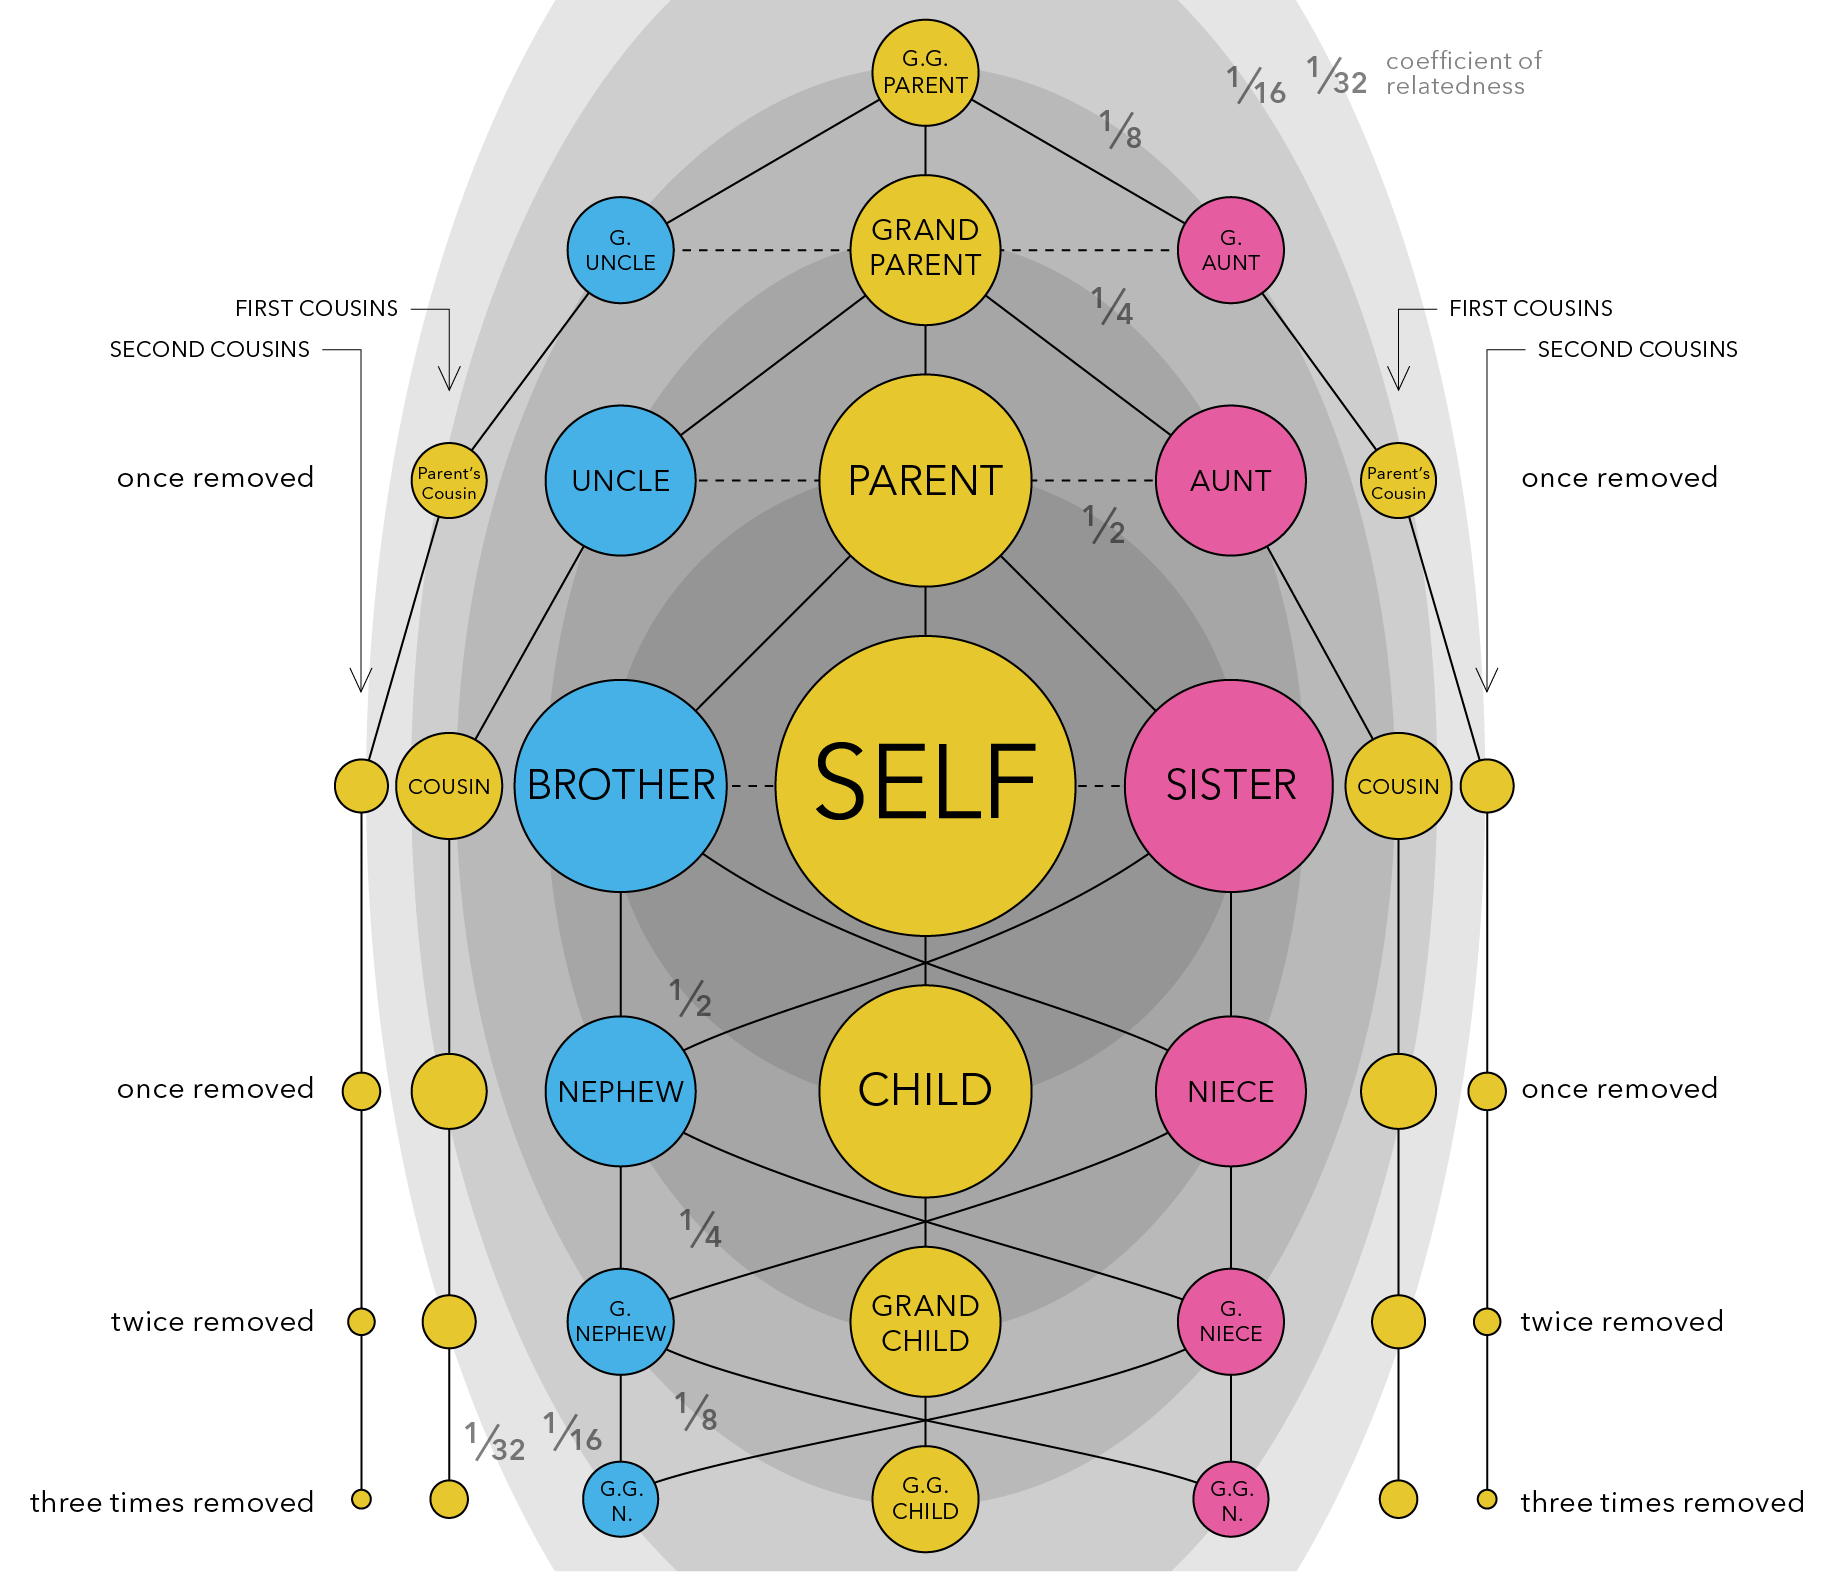
\includegraphics[width=0.5\textwidth]{coefrelate.png}
	\caption{Wright's coeffcient of relatedness by Citynoise - Own work, CC BY-SA 4.0, \url{https://commons.wikimedia.org/w/index.php?curid=37723128}}
	\label{fig:coefrelate}
\end{figure}
\par
% Richard Dawkins~\cite{selfish_gene} advocated for the idea of the selfish gene. From a biological perspective, this idea postulates that actors are hardwired to propagate their genes. Dawkins asserts that this drive is due to the fact that genes are the true replicators evolutionarily rather than the actors themselves. Those with a high coefficient of relatedness to an individual are far more likely to carry their genes and to help them proliferate. This mechanism is similar to that presented by Hamilton~\cite{kinhamilton}, but with a biological backing. From a biological perspective this may make sense. However, it does not seem natural to translate an agent's strategy to the idea of genes.\par
% Further, although it is possible to create a coefficient and an idea of relatedness similar to that of Hamilton's model~\cite{kinhamilton} for a MAS, it does not seem a natural translation. Another limitation to the use of kinship theory for MASs is that systems are ideally inclusive of individuals that can contribute to the society. For example, if an agent is looking to actively contribute to a society, but is not kin with the members, a MAS using kinship theory would exclude them and thus limit the abilities of that society.\par
% Furthermore, Axelrod and Hamilton~\cite{evolution_of_cooperation} highlight that humanity is the exceptional society which does not limit itself to cooperating mostly only with kin. I would surmise that this exception is due to the higher level of intellect of homo-sapiens in comparison to other species. Many have suggested that the capabilities of AI could match or even surpass the intelligence of humans. Therefore, I would suggest that societies of IAs should also not be limited to the use of kinship theory to facilitate cooperation.\par
% As such, I shall not be using kinship theory for my theoretical framework. I will be aiming to use a  mechanism that is inclusive of agents that aim to become valuable members of the society and also a mechanism which fits naturally into the agent's paradigm. 
\begin{figure}
	\center
	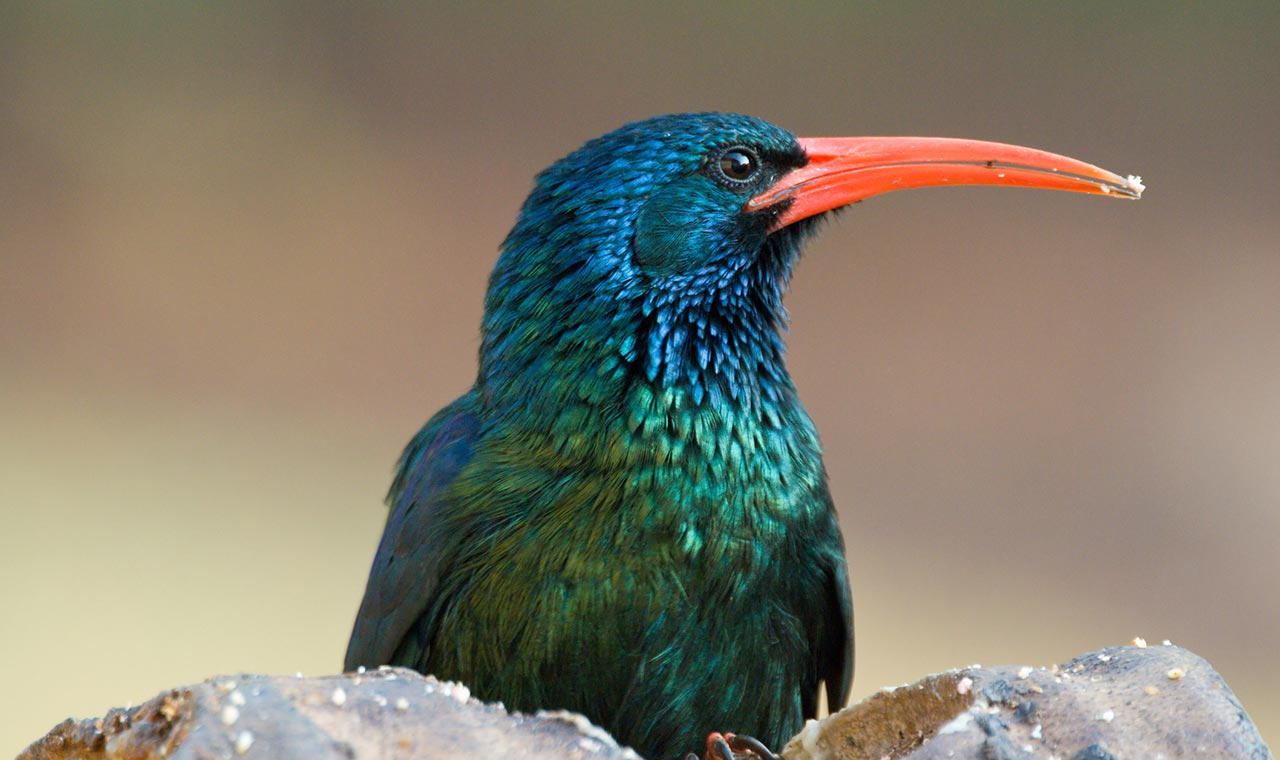
\includegraphics[width=0.5\textwidth]{green-wood-hoopoe.jpg}
	\caption{The Green Wood-Hoopoe native to Africa participates in cooperative breeding as the bird not only looks after its own chicks, but those of other breeding pairs~\cite{hoopoe}}
	\label{fig:hoopoe}
\end{figure}

\subsection{Network Reciprocity}
\label{appendix:netreciprocity}
% Nowak - in his paper `The Five Rules of Cooperation'~\cite{five_rules_coop} - identified and compared five key mechanisms that can aid in the evolution of cooperation, two of which I have already discussed (direct reciprocity in section~\ref{sec:ipd} and kin selection in ~\ref{sec:kin}). The other three are network reciprocity (which I shall examine here), group selection and indirect reciprocity (both of which have their own sections).\par
% Network reciprocity uses a graph of players and their connections. The players are represented by the nodes in the graph, with arcs representing connections between players. This idea ties closely to the networks that IAs may work across. Players with arcs between them interact with each other in rounds of The Prisoner's Dilemma. Nowak and May's~\cite{spatial} ealier work - which inspired Nowak's later paper~\cite{five_rules_coop} - did not give individual's any memory of past interaction.\par
% This lack of memory limited Nowak and May to pure cooperators and pure defectors. In Nowak's book `Evolutionary Dynamics'~\cite{nowak2006evolutionary}, his exploration of evolutionary graph theory and spatial games (chapters 8 and 9) showed that the shapes of the lattice linking the players and different concentrations of cooperators and defectors on those shapes has a great effect on the evolution of cooperation. Visualised in figures~\ref{fig:coopinvdef} and ~\ref{fig:funnel}.\par
% Nowak's~\cite{five_rules_coop, nowak2006evolutionary} and Nowak and May's~\cite{spatial} work on these games on graphs is limited in terms of strategies and also in terms of the fixed shape of its graphs. However, the work proves a key point: the structure of who interacts with whom can play a key role in supporting cooperation in large populations.\par
% In real life, individuals will often mostly interact in their close social circles. For example, a Meerkat may interact with others of their family group, a drongo bird which calls to warn of predators, the predators and others who are geographically close to them. The graph in this case represents the close geographic ties.\par
% I imagine the use of Nowak~\cite{five_rules_coop, nowak2006evolutionary} and Nowak and May's~\cite{spatial} work to employ a network not as a representation of a physical network structure or geography, but as a representation of the choices made by IAs with whom they wish to interact with.\par
% This network would be a constantly changing and adapting network of IAs. The IAs would not concern themselves with the strategy they employ towards whom they are forced to interact with. Instead, their strategy is to select those whom they wish to interact with, thus, effectively constructing a graph of network reciprocation. How these changing graph connections would affect cooperation is unbeknownst to me. Indeed, whether Nowak's rules would still apply would be interesting to find out.\par
% Nowak~\cite{nowak2006evolutionary} found that some shapes supported cooperators in groups. Cooperators could make use of these shapes by deliberately forming them to protect one another. While another set of shapes were found as `amplifiers' for evolution, maybe defectors could make use of these sorts of shapes to invade groups of cooperators.\par
% I can see IAs having strategies as to how to build these shapes. However, an issue may arise in which cooperative agents find it hard to reach out to other cooperators which are not part of their current shape.As such, there may be possible prevention of the spread of cooperation, thus limiting these groups. However, this concept is worth investigating, and the problem could possibly be overcome using some kind of bridging mechanism.\textcolor{red}{Compare to \cite{jennings2000agent} organisational relationships}.
\begin{framed}
	\begin{center}
		\begin{tabular}{c|cc}
		& \textcolor{blue}{A} & \textcolor{red}{B}\\	
		\hline
		\textcolor{blue}{A} & a & b\\
		\textcolor{red}{B} & c & d\\
		\end{tabular}
		\captionof{table}{The payoff matrix for when individuals interact. Cooperators are in blue and are called A, and defectors in red and called B. Taken from Nowak's book Evolutionary Dynamics~\cite{nowak2006evolutionary}.}
		\label{tab:networkmatrix}
	\end{center}	
\end{framed}
\begin{figure}
	\center
	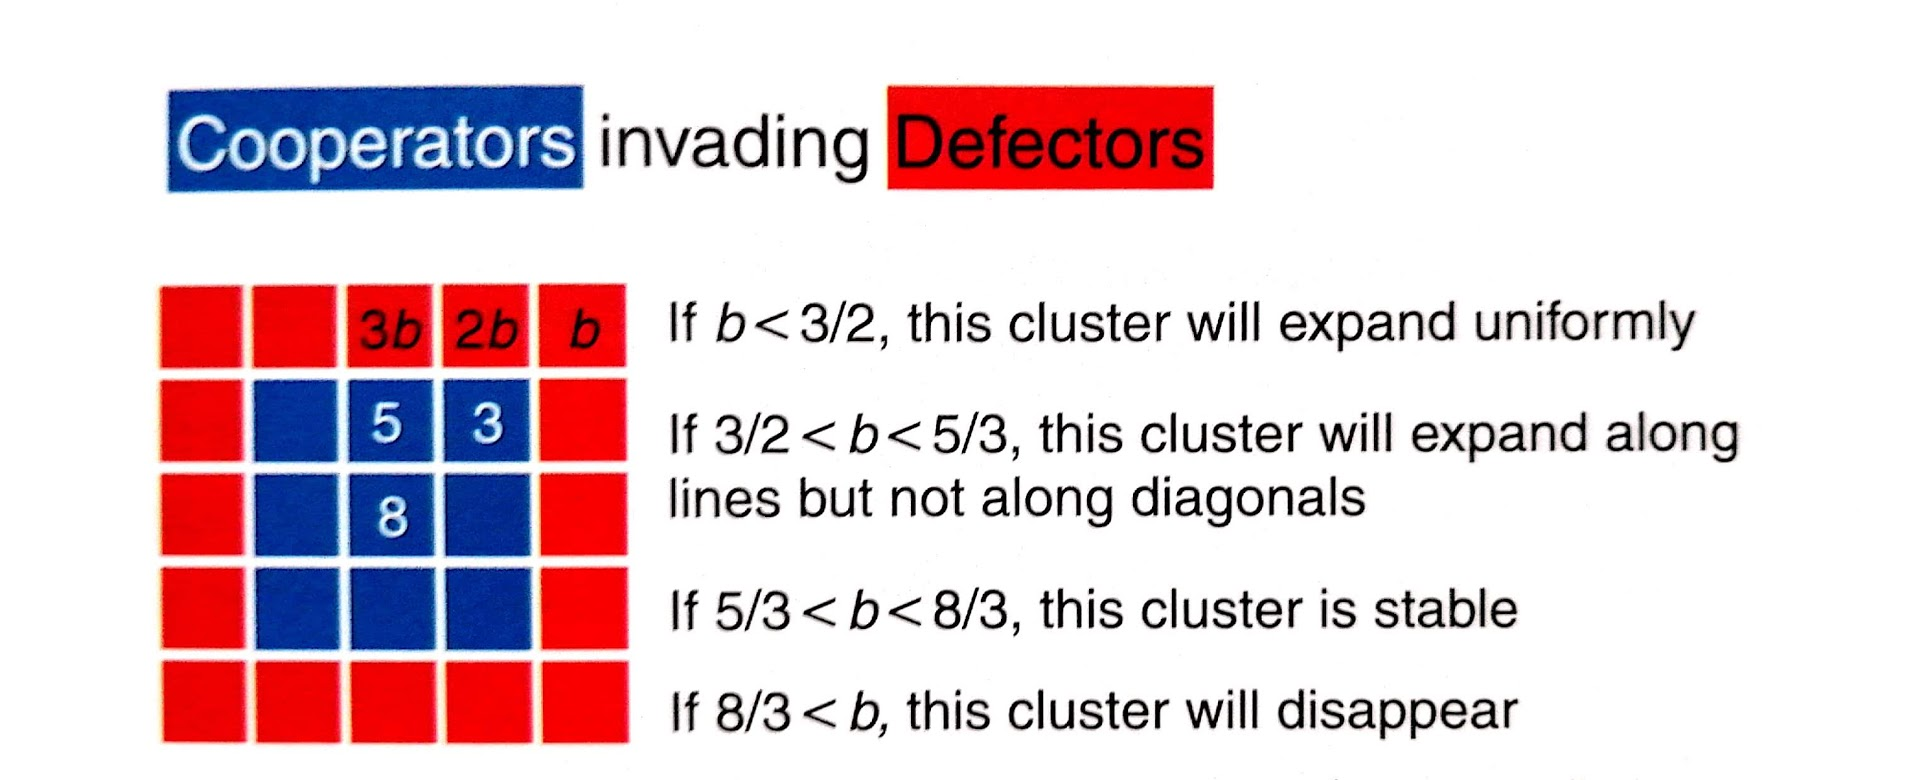
\includegraphics[width=0.5\textwidth]{cooperators-invading-defectors.jpg}
	\caption{How can cooperators invade defectors? Taken from Nowak's book Evolutionary Dynamics~\cite{nowak2006evolutionary}. The squares represent nodes and the players interact with the players to each side of them and diagonally. The value b is from the payoff matrix in table~\ref{tab:networkmatrix}}
	\label{fig:coopinvdef}
\end{figure}
\begin{figure}	\center
	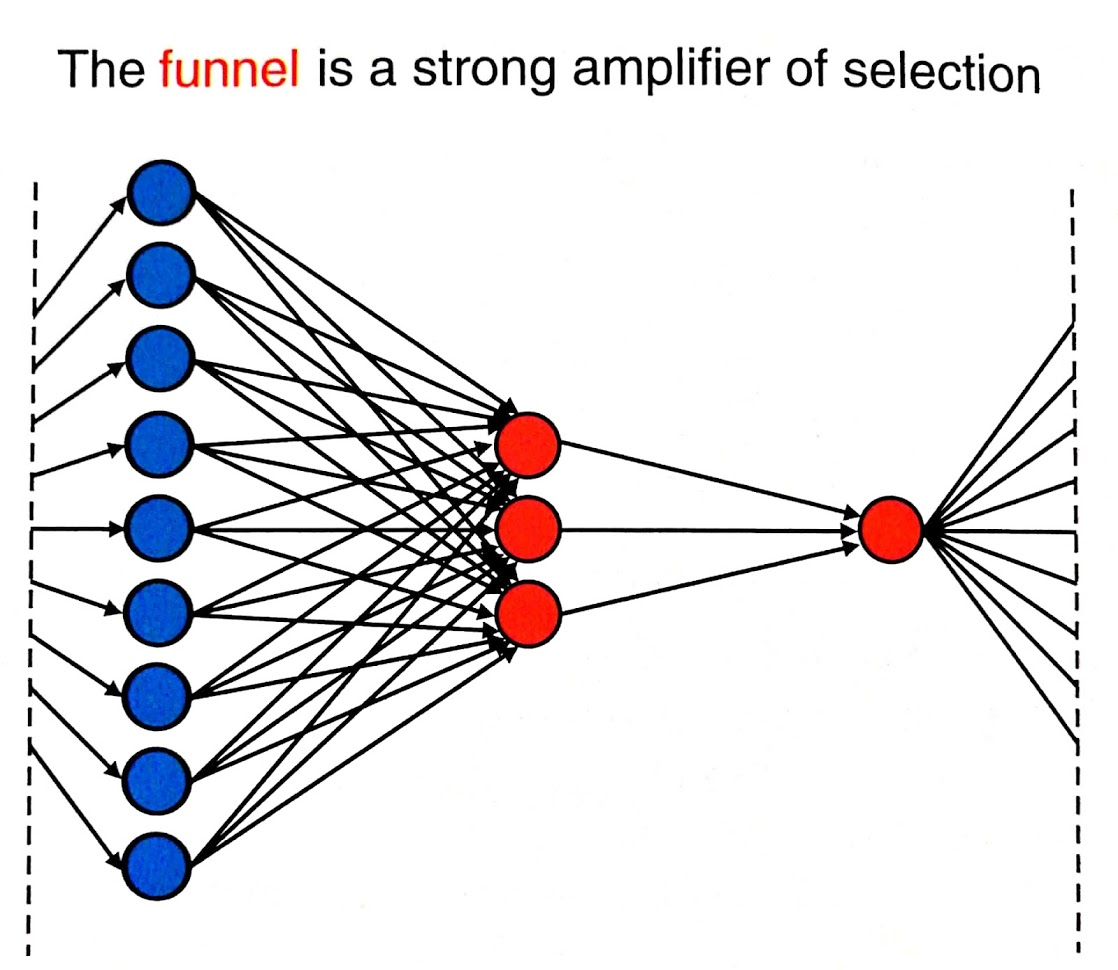
\includegraphics[width=0.5\textwidth]{funnel_amplifier.jpg}
	\caption{Shapes that can amplify selection include the funnel, the star and the superstar~\cite{nowak2006evolutionary}}
	\label{fig:funnel}
\end{figure}


\subsection{Group Selection}
\label{appendix:groupselection}
% Group selection is another mechanism described by Nowak~\cite{five_rules_coop}. This mechanism splits one population into multiple groups. Within these groups, The Prisoner's Dilemma is played and reproduction occurs which is proportional to each players payoff. If using the payoff matrix in table~\ref{tab:payoffmatrix}, then cooperators can work together to produce a payoff of three, while defectors can only produce five or two for both players in the interaction.\par
% The group size increases until a certain point, at which the group may split. If the group does split (which is stochastically chosen) then another group is destroyed. The effect is multi-level selection.\par
% Nowak found that due to the higher payoff between cooperators, reproduction will occur more quickly within the groups they dominate, than the groups filled with defectors. The faster the reproduction, the quicker the group size grows, making it more likely for groups of cooperators to survive while groups of defectors will shrink and be destroyed. These dynamics are displayed in figure~\ref{fig:group}.\par
% Traulsen and Nowak~\cite{multilevel_nowak} limited themselves to cooperators and defectors, but noted that other strategies could be built into their model. A limitation to applying group selection to MASs is the groups themselves. In this model, individuals do not interact with individuals in other groups, creating a barrier between them.\par
% Even our current networks span the globe and don't always have harsh barriers between them - even when security is high, these barriers can often be broken. Furthermore, IAs are often built to be of service to others and limiting them to being of service only to one group greatly reduces the service an agent can supply and limits the society as a whole . Finally, the group mechanics of splitting and destroying another group of individuals does not naturally match the paradigm of MASs.\par
% I would suggest that this is not a mechanism which would be useful to apply to MASs unless you are modelling clusters of agents, with each cluster in competition. This idea is not the aim of my project; however it could be another interesting project to take up.
\begin{figure}
	\center
	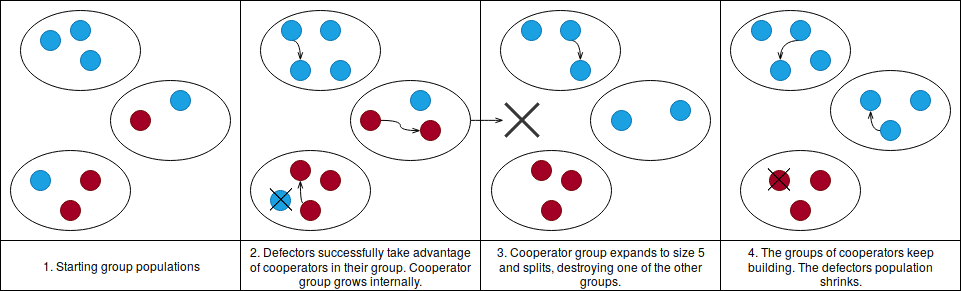
\includegraphics[width=\textwidth]{GroupSelection.png}
	\caption{The dynamics of multi-level selection as described by Traulsen and Nowak~\cite{multilevel_nowak}.}
	\label{fig:group}
\end{figure}
\subsection{Alternate Agent Architectures}

\section{Theoretical Framework}
\subsection{Environment Properties}
\label{appendix:envprop}
% I have already discussed how the synchronised cycle steps makes my environment static, but what about Russell and Norvig's~\cite{russell2016artificial} 4 other properties. Knowing the intention of other agents is key to deciding on whether other agents should cooperate or not. However, agents cannot view all interactions, and gossip may be distorted so an agent may not know all details it needs to know for action decisions. As such, the environment I have delineated is only partially observable.\par
% I also argue that the environment is deterministic from a generational point of view. Milinski \textit{et al.}~\cite{imagevsstanding} claimed that individuals using the standing strategy aim for a good standing, and Leimar and Hammerstein~\cite{leimarhammer} argue that the standing strategy is good as it allows individuals to punish bad individuals. However take 3 agents a, b, c and d. Agent b has defected previously against d who has a good standing according to a. Agent a then chooses to punish b but is still believing this won't reduce their standing. However, agent c did not observe b's defection against d but is an onlooker for c's defection against b.\par
% From the proceedings the environment appears to be non-deterministic, as there is more than one outcome to an action. However, this is due to the partial observability of the environment not the determinism, as highlighted is possible by Russell and Norvig~\cite{russell2016artificial}. The current state (c's lack of knowledge on b) and the actions selected by a and b completely determine the next state of the system.\par
% However, from a community point of view the game can be seen as non-deterministic due to the reproduction mechanism. This includes a chance of mutation and the actual selection of agents is stochastic. As such the actions of the agents cannot guarantee that their strategy will be highly propagated, the higher the fitness they get (which is decided by state and actions) affects their chances greatly but not fully.\par
% The environment is also nonepisodic. To take a proof by contradiction approach suppose the environment is episodic. According to Russell and Norvig~\cite{russell2016artificial} an environment is episodic if subsequent episodes do not depend on what action occurs in previous episodes. Episodes consist of perceiving and then deciding. But from the percepts and actions subsections (\ref{subs:percepts} and \ref{subs:actions}) we know that actions from one timepoint can generate percepts in the next. This is a contradiction and as such the environment is nonepisodic.\par
% In summary the environment I have outlined in this section is inaccessible, deterministic from a generational point of view yet non-deterministic from a community point of view, nonepisodic, static and discrete.
\subsection{Strategies}
\label{appendix:strats}
\textcolor{red}{include list of strategy components and trust models, all associated together}.

\end{document}
